In diesem abschließenden Kapitel möchten wir die Ergebnisse der in
\Cref{chap:implementation} beschriebenen Realisierung von
\Cref{alg:primalDualIteration} mit Abbruchkriterium
\eqref{eq:terminationCriterion} im Solve-Schritt der AFEM-Schleife aus
\Cref{fig:afemLoop} untersuchen, deren initiales Level dabei mit 0 nummeriert
wird.
Bezüglich einer Triangulierung $\Tcal$ schreiben wir hier $\ucrt$ und
$\bar\Lambda_{0,\Tcal}$ für $\ucr$ und $\bar\Lambda_0$ aus
\Cref{thm:convergenceIteration} sowie $(\ujt, \Lambda_{j,\Tcal})_{j\in\Nbb}$
für die Iterate $\left(u_j, \Lambda_j\right)_{j\in\Nbb}$  von
\Cref{alg:primalDualIteration}.
Zunächst möchten wir die Belegung für alle Parameter aus den Tabellen
\ref{tab:paramsMisc}--\ref{tab:paramsExperiment}, die für ein Experiment
relevant sind, festlegen.
Die Wahlen $\tau = 1$ für \Cref{alg:primalDualIteration} und $\epsstop
= 10^{-4}$ für das Abbruchkriterium \eqref{eq:terminationCriterion} begründen
wir in \Cref{sec:choiceOfParameters} experimentell. 
Außerdem nutzen wir $\gamma = 1$ für den Parameter $\gamma$ des
Verfeinerungsindikators aus \Cref{def:refinementIndicator}, wobei wir den
Einfluss dieses Parameters auf das Programm in
\Cref{sec:experimentsWithExactSolution} untersuchen. 
Eine Übersicht über alle somit festgelegten Standardwerte ist in
\Cref{tab:parameterStandardValues} zu finden. 
Wir werden in einem Experiment die Wahl eines Parameters nur
erwähnen, wenn diese vom Standardwert abweicht.
In \Cref{tab:usedBenchmarks} wird für alle verwendeten Benchmark-Dateien
aufgelistet, für welche Abbildungen die Ergebnisse des entsprechenden
Programmaufrufs genutzt wurden.

\begin{table}[p]
  \centering
  \begin{tabular}{c|p{9.5cm}}
    \hline 
    Parametername & Standardwert\\
    \hline 
    \texttt{degree4Integrate}&
    $10$\\
    \texttt{geometry} &
    \texttt{'BigSquare'} für Experimente mit bekannter exakter Lösung \newline
    \texttt{'Square'} für Experimente mit Graufarbenbild als Eingangssignal\\
    \texttt{initialRefinementLevel} &
    $0$\\
    \texttt{parTheta}, $\theta$ &
    $0.5$\\
    \texttt{minNrDof} &
    $10^8$\\
    \texttt{useProlongation} &
    \texttt{true}\\
    \texttt{parGamma}, $\gamma$ &
    $1$\\
    \texttt{d}, $d$ &
    $2$\\
    \texttt{u0Mode} &
    \texttt{zeros}\\
    \texttt{epsStop}, $\epsstop$ &
    $10^{-4}$\\
    \texttt{parTau}, $\tau$ &
    $1$\\
    \texttt{maxIter} &
    $10^{12}$\\
    \texttt{parAlpha}, $\alpha$ &
    $\alpha$ für Experimente mit Eingangssignal $f_\alpha$\newline
    $10^4$ für Experimente mit Eingangssignal \texttt{cameraman} \\
    \texttt{parBeta}, $\beta$ &
    $1$ für Experimente mit Eingangssignal $f_\alpha$\\
    \hline
  \end{tabular}
  \caption{Wahl der relevanten Parameter für die Experimente}
  \label{tab:parameterStandardValues}
\end{table} 
\begin{table}[p]
  \centering
  \begin{tabular}{c|p{8.7cm}}
    \hline
    \texttt{benchmark} & Abbildungen\\  
    \hline 
    \texttt{denoiseAlpha100} &
    \ref{fig:snr15alpha100}, \ref{fig:denoiseConvergence},
    \ref{fig:denoiseNrIterComparison}\\
    \texttt{denoiseAlpha1000} &
    \ref{fig:snr15alpha1000}, \ref{fig:denoiseConvergence},
    \ref{fig:denoiseNrIterComparison}\\
    \texttt{denoiseAlpha2500} &
    \ref{fig:snr15alpha2500}\\
    \texttt{denoiseAlpha5000} &
    \ref{fig:snr15alpha5000}\\
    \texttt{denoiseAlpha10000} &
    \ref{fig:snr15alpha10000}, \ref{fig:denoiseConvergence}, 
    \ref{fig:denoiseNrIterComparison}\\
    \texttt{denoiseAlpha50000} &
    \ref{fig:snr15alpha50000}\\
    \texttt{paramsTau\_f01\_0Dot1} &
    \ref{fig:parTauMiscF}, \ref{fig:parTauConvergence},
    \ref{fig:iterationEnergyOscillations}\\
    \texttt{paramsTau\_f01\_0Dot5} &
    \ref{fig:parTauMiscF}, \ref{fig:parTauConvergence}\\
    \texttt{standard\_f01} &
    \ref{fig:parTauMiscF}, \ref{fig:parTauConvergence}, 
    \ref{fig:iterationEnergyLevel}, \ref{fig:iterationTermination},
    \ref{fig:f01SolAdaptive}, \ref{fig:f01Convergence}, 
    \ref{fig:f01SupplementaryInfo}, \ref{fig:parGammaConvergence},
    \ref{fig:gamma1Triang}, \ref{fig:inSiNrIterComparison},
    \ref{fig:miscF01}\\
    \texttt{paramsTau\_cameraman\_0Dot1} &
    \ref{fig:parTauMiscCam}\\
    \texttt{paramsTau\_cameraman\_0Dot5} &
    \ref{fig:parTauMiscCam} \\
    \texttt{standard\_cameraman} &
    \ref{fig:parTauMiscCam}, \ref{fig:camConvergence}, \ref{fig:camTriang},
    \ref{fig:miscCam}\\
    \texttt{noTerminationTau\_maxIter1e5} &
    \ref{fig:parTauNoConvergence}\\
    \texttt{paramsEpsStop\_1em2} &
    \ref{fig:parEpsStopConvergence}, \ref{fig:triangEpsStop1em2}\\
    \texttt{paramsEpsStop\_1em3} &
    \ref{fig:parEpsStopConvergence}\\
    \texttt{paramsEpsStop\_1em4} &
    \ref{fig:parEpsStopConvergence}\\
    \texttt{paramsEpsStop\_1em5} &
    \ref{fig:parEpsStopConvergence}, \ref{fig:triangEpsStop1em5}\\
    \texttt{standardUniform\_f01} &
    \ref{fig:f01Convergence}, \ref{fig:f01SupplementaryInfo},
    \ref{fig:miscF01}\\
    \texttt{standard\_f04} &
    \ref{fig:f04Convergence}, \ref{fig:inSiNrIterComparison}\\
    \texttt{standardUniform\_f04} &
    \ref{fig:f04Convergence}\\
    \texttt{paramsGamma\_0} &
    \ref{fig:parGammaConvergence}, \ref{fig:gamma0Triang}\\
    \texttt{paramsGamma\_1em2} &
    \ref{fig:parGammaConvergence}\\
    \texttt{paramsGamma\_0Dot5} &
    \ref{fig:parGammaConvergence}, \ref{fig:gammaDot5Triang}\\
    \texttt{standard\_f01Alpha1e4} &
    \ref{fig:f01LargeAlphaConvergence}, \ref{fig:inSiNrIterComparison}\\
    \texttt{standardUniform\_f01Alpha1e4} &
    \ref{fig:f01LargeAlphaConvergence}\\
    \texttt{standardUniform\_cameraman} &
    \ref{fig:camConvergence}, \ref{fig:miscCam}\\
    \texttt{circleContinuousAdaptive} &
    \ref{fig:circConvAdaptive}, \ref{fig:circContLvl17Triang},
    \ref{fig:circContSol}, \ref{fig:circContSolAxis}, 
    \ref{fig:circContConvergence}, \ref{fig:miscCircle}\\
    \texttt{circleDiscontinuousAdaptive} &
    \ref{fig:circConvAdaptive}\\
    \texttt{circleContinuousUniform} &
    \ref{fig:circConvUniform}, \ref{fig:circDiscLvl17Triang},
    \ref{fig:circDiscSol}, \ref{fig:circDiscSolAxis},
    \ref{fig:circContConvergence}, \ref{fig:miscCircle}\\
    \texttt{circleDiscontinuousUniform} &
    \ref{fig:circConvUniform}\\
    \hline
  \end{tabular}
  \caption{Eingabeparameter \texttt{benchmark} für \texttt{startAlgorithmCR},
    um die Rechnung zu einem Experiment zu starten, und die Abbildungen, die
    auf den Ergebnissen dieses Experiments basieren} 
  \label{tab:usedBenchmarks}
\end{table} 

Als Startwert für die primale-duale Iteration des ersten Levels der
AFEM-Routine wählen wir $u_0\equiv 0$. 
Für die Iteration der darauffolgenden Level wählen wir die zum Ende von
\Cref{sec:programFlow} beschriebene Prolongation des Ergebnisses des
jeweils vorherigen Levels.
In allen Experimenten hatte dadurch die Wahl des Startwerts für die Iteration
des ersten Levels keinen nennenswerten Einfluss auf die Dauer des Experiments
oder die Güte der Ergebnisse. 
Für jeden Aufruf der primalen-dualen Iteration auf einer Triangulierung $\Tcal$
wählen wir dann $\Lambda_{0,\Tcal}$ wie in
\Cref{eq:choiceInitialDualVariableImplementation} angegeben.
Eingangssignale für Experimente, bei denen die exakte
Lösung bekannt ist, konstruieren wir nach \Cref{sec:constructionInputSignal}.
Die schwachen Ableitungen dieser Eingangssignale und der entsprechenden exakten
Lösungen berechnen wir ebenfalls nach \Cref{sec:constructionInputSignal}.
Dabei sei das Argument $r$ einer Funktion stets aus $[0,\infty)$.
\begin{figure}[p]
  \centering
  \begin{subfigure}[b]{.48\linewidth}
    \centering
    \caption{\texttt{BigSquare}}
    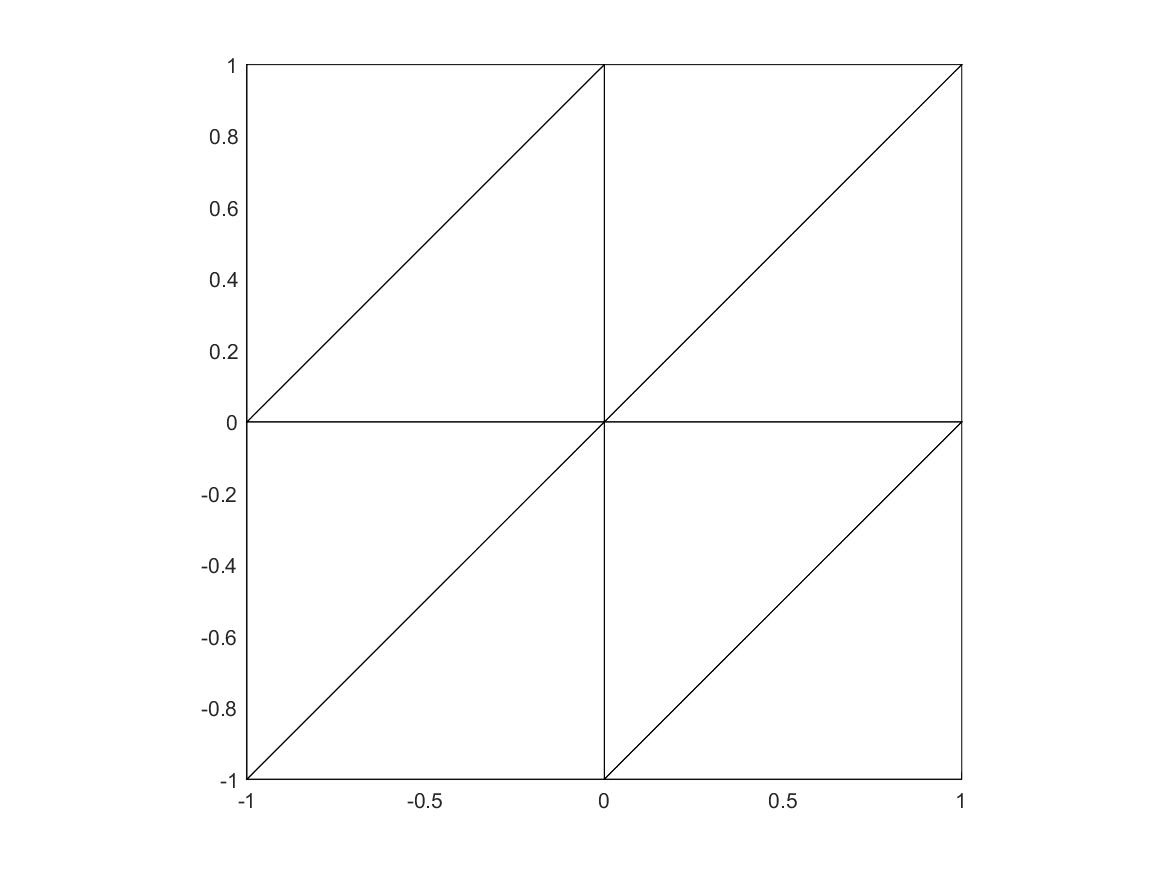
\includegraphics[trim = 90 30 90 20, clip, width=\linewidth]
      {pictures/chapExperiments/secGeneralInfo/bigSquareTriang.png}
    \label{fig:triangBigSquare}
  \end{subfigure}
  \quad
  \begin{subfigure}[b]{.48\linewidth}
    \centering
    \caption{\texttt{Square}}
    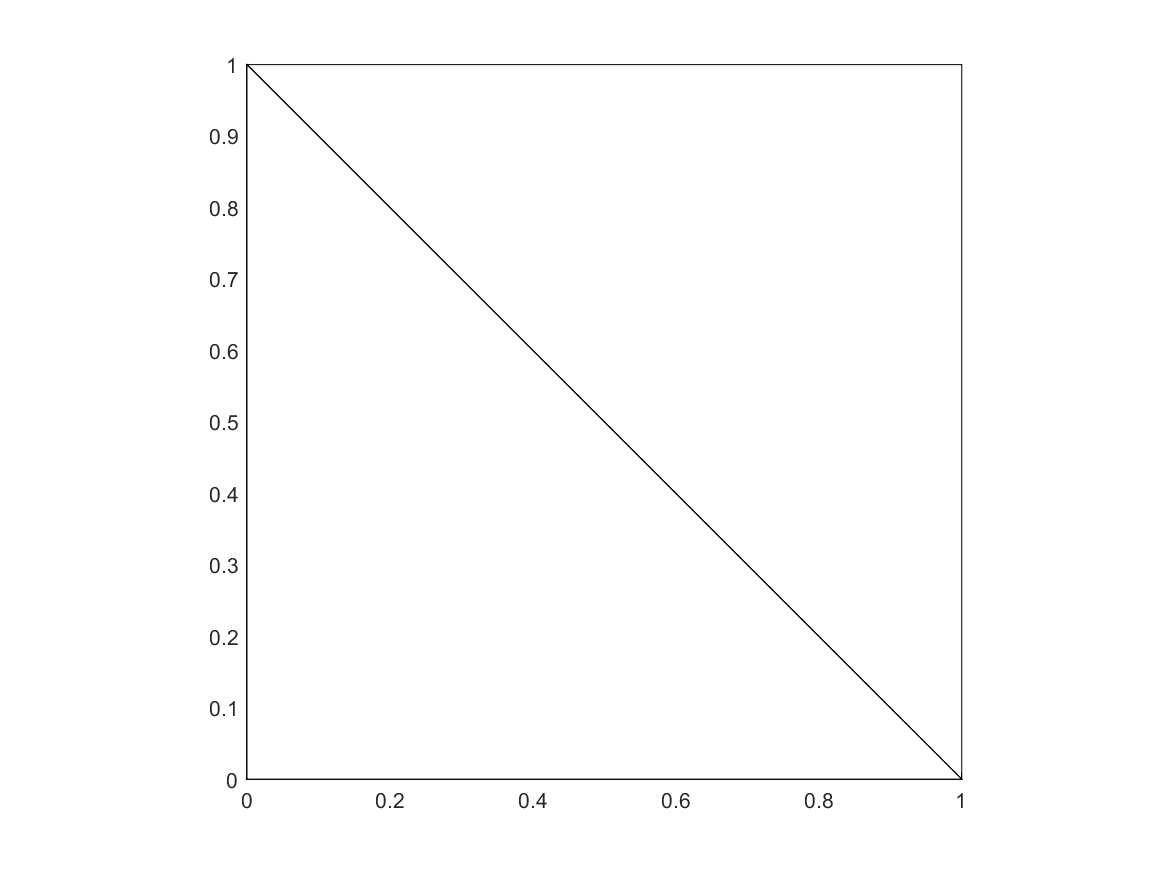
\includegraphics[trim = 90 30 90 20, clip, width=\linewidth]
      {pictures/chapExperiments/secGeneralInfo/squareTriang.png}
    \label{fig:triangSquare}
  \end{subfigure}
  \caption{Initiale Triangulierung für Experimente mit bekannter exakter Lösung
    (a) und initiale Triangulierung für Experimente mit Graufarbenbild als
    Eingangssignal (b)}
  \label{fig:initialTriangulations}
\end{figure}
Als Geometrie für das erste Level des AFEM-Al\-go\-rith\-mus nutzen wir in
Experimenten mit bekannter exakter Lösung die Triangulierung aus
\Cref{fig:triangBigSquare} und in Experimenten mit einem Graufarbenbild als
Eingangssignal die Triangulierung aus \Cref{fig:triangSquare}.
Wir nutzen adaptive Netzverfeinerungen und dafür den Bulk-Parameter
$\theta=0.5$ für den Mark-Schritt des AFEM-Algorithmus und den Parameter
$\gamma=1$ für den Verfeinerungsindikator aus \Cref{def:refinementIndicator}.
Die maximale Iterationszahl wurde mit $10^{12}$ so gewählt, dass diese nie
Grund für das Beenden der primalen-dualen Iteration war.
Dementsprechend ist das Abbruchkriterium aus \eqref{eq:terminationCriterion}
für den Abbruch der Iteration verantwortlich.
Die minimale Anzahl der Freiheitsgrade, welche eine Triangulierung während der
AFEM-Routine zum Abbrechen erreichen soll, ist mit $10^8$ so gewählt, dass die
verfügbaren Ressourcen des verwendeten Rechners in der Regel ausgenutzt
werden und die Rechnungen manuell beendet werden müssen.
Dies geschah in allen Experimenten bei ungefähr $10^6$ Freiheitsgraden.
Beispielrechnungen mit verschiedenen Eingangssignalen ergaben, dass deutlich
höhere Integrationsgrade als $10$ zu keinen veränderten Konvergenzraten
führen. 
Diese Wahl des Integrationsgrads erscheint daher als ausreichend.
Da außerdem die Methode \texttt{integrate} des AFEM-Softwarepakets \cite{Car09}
nicht während der primalen-dualen Iteration aufgerufen werden muss, hat eine
möglicherweise zu hohe Wahl des Integrationsgrads keinen signifikanten Einfluss
auf die Programmlaufzeit.
Nur die Methode \texttt{errorCRL2} des AFEM-Softwarepakets, die zur Berechnung
des exakten $L^2$-Fehlers verwendet wird, nutzt den Integrationsgrad 12, da
diese unverändert übernommen wurde.

Nun möchten wir ein Eingangssignal definieren, welches in mehreren der
folgenden Abschnitte verwendet wird.
Sei $\beta\geq 1/2$, wobei wir stets $\beta=1$ wählen. 
Wir betrachten die Funktion
\begin{align*}
  u(r)&\coloneqq
  \begin{cases}
    1, 
    & \text{falls } r\in \left[0,\frac{1}{6}\right]\!,\\
    1+(6r-1)^\beta, 
    & \text{falls } r\in \left(\frac{1}{6}, \frac{1}{3}\right]\!,\\
    2, 
    & \text{falls } r\in \left(\frac{1}{3}, \frac{1}{2}\right]\!,\\
    2\left(\frac{5}{2}-3r\right)^\beta, 
    & \text{falls } r\in \left(\frac{1}{2}, \frac{5}{6}\right]\!,\\
    0, 
    & \text{falls } r\in \left(\frac{5}{6}, \infty\right)\!,\\
  \end{cases}
\end{align*}
und wählen
\begin{align*}
  \sgn\big(\partial_r u(r)\big) 
  &\coloneqq
  \begin{cases}
    12r-36r^2, 
    & \text{falls } r\in \left[0,\frac{1}{6}\right]\!,\\
    1, 
    & \text{falls } r\in \left(\frac{1}{6}, \frac{1}{3}\right]\!,\\
    \cos(\pi(6r-2)), 
    & \text{falls } r\in \left(\frac{1}{3}, \frac{1}{2}\right]\!,\\
    -1, 
    & \text{falls } r\in \left(\frac{1}{2}, \frac{5}{6}\right]\!,\\
    -\frac{1+\cos(\pi(6r-5))}{2}, 
    & \text{falls } r\in \left(\frac{5}{6}, \infty\right)\!.
  \end{cases}
\end{align*}
Nach \Cref{eq:constructionInputSignal} ist $u$ mit dieser Wahl von
$\sgn\big(\partial_r u\big)$ die Lösung von \Cref{prob:continuousProblem} mit
Eingangssignal
\begin{align*}
  f_\alpha(r)
  &=
  \begin{cases}
    \alpha-12(2-9r), 
    & \text{falls } r\in \left[0,\frac{1}{6}\right]\!,\\
    \alpha\left(1+(6r-1)^\beta\right)-\frac{1}{r}, 
    & \text{falls } r\in \left(\frac{1}{6}, \frac{1}{3}\right]\!,\\
    2\alpha+6\pi\sin(\pi(6r-2))-\frac{1}{r}\cos(\pi(6r-2)), 
    & \text{falls } r\in \left(\frac{1}{3}, \frac{1}{2}\right]\!,\\
    2\alpha\left(\frac{5}{2}-3r\right)^\beta+\frac{1}{r},
    & \text{falls } r\in \left(\frac{1}{2}, \frac{5}{6}\right]\!,\\
    -3\pi\sin(\pi(6r-5))+\frac{1+\cos(\pi(6r-5))}{2r}, 
    & \text{falls } r\in \left(\frac{5}{6}, \infty\right)\!.
  \end{cases}
\end{align*}
Dieses Eingangssignal für zwei Wahlen von $\alpha$ und die exakte Lösung $u$
von \Cref{prob:continuousProblem} mit Eingangssignal $f_\alpha$ können in
\Cref{fig:f01Plots} betrachtet werden.
Wir können anhand von \Cref{fig:f01Plots} ebenfalls den in
\Cref{chap:introduction} beschriebenen Zusammenhang von
\Cref{prob:continuousProblem} und dem ROF-Modell sehen, denn für $\alpha=10^4$
scheint annähernd $f_\alpha=\alpha u$ zu gelten.
\begin{figure}[p]
  \centering
  \begin{subfigure}[b]{.48\linewidth}
    \centering
    \caption{$f_1$}
    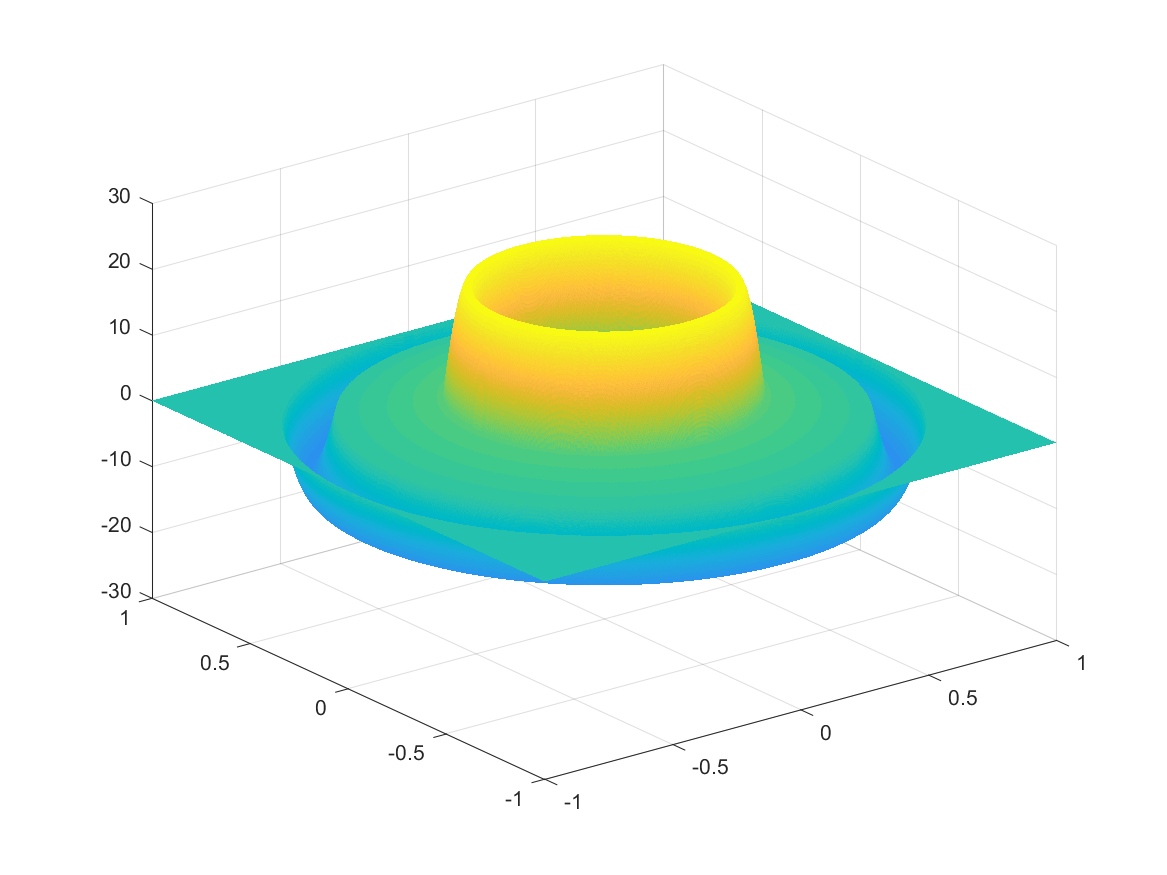
\includegraphics[trim = 40 30 30 30, clip, width=\linewidth]
      {pictures/chapExperiments/secGeneralInfo/f01Plots/inSi1.png}
    \label{fig:f01InSi}
  \end{subfigure}
  \quad
  \begin{subfigure}[b]{.48\linewidth}
    \centering
    \caption{$f_1$ entlang der x- und y-Achse}
    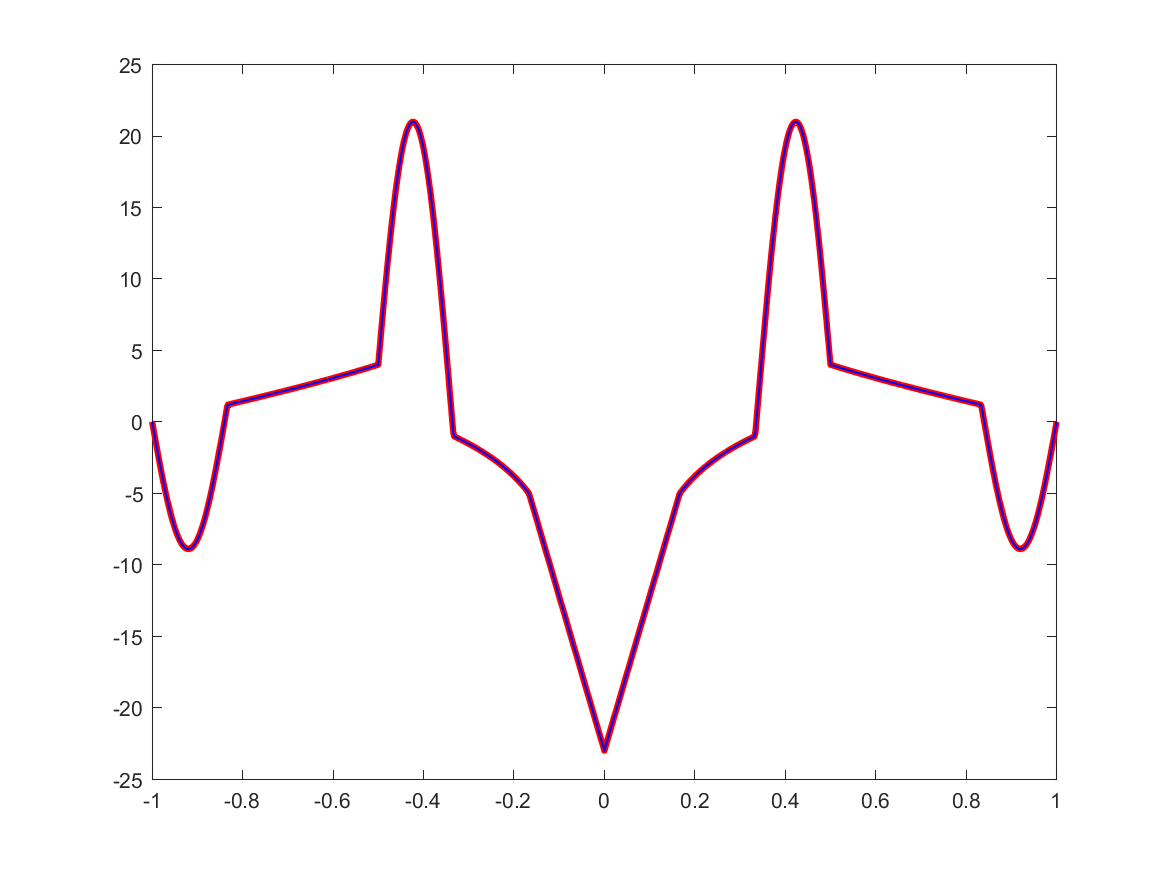
\includegraphics[trim = 50 30 50 20, clip, width=\linewidth]
      {pictures/chapExperiments/secGeneralInfo/f01Plots/inSi1Axis.png}
    \label{fig:f01InSiAxis}
  \end{subfigure}

  \begin{subfigure}[b]{.48\linewidth}
    \centering
    \caption{$f_{10^4}$}
    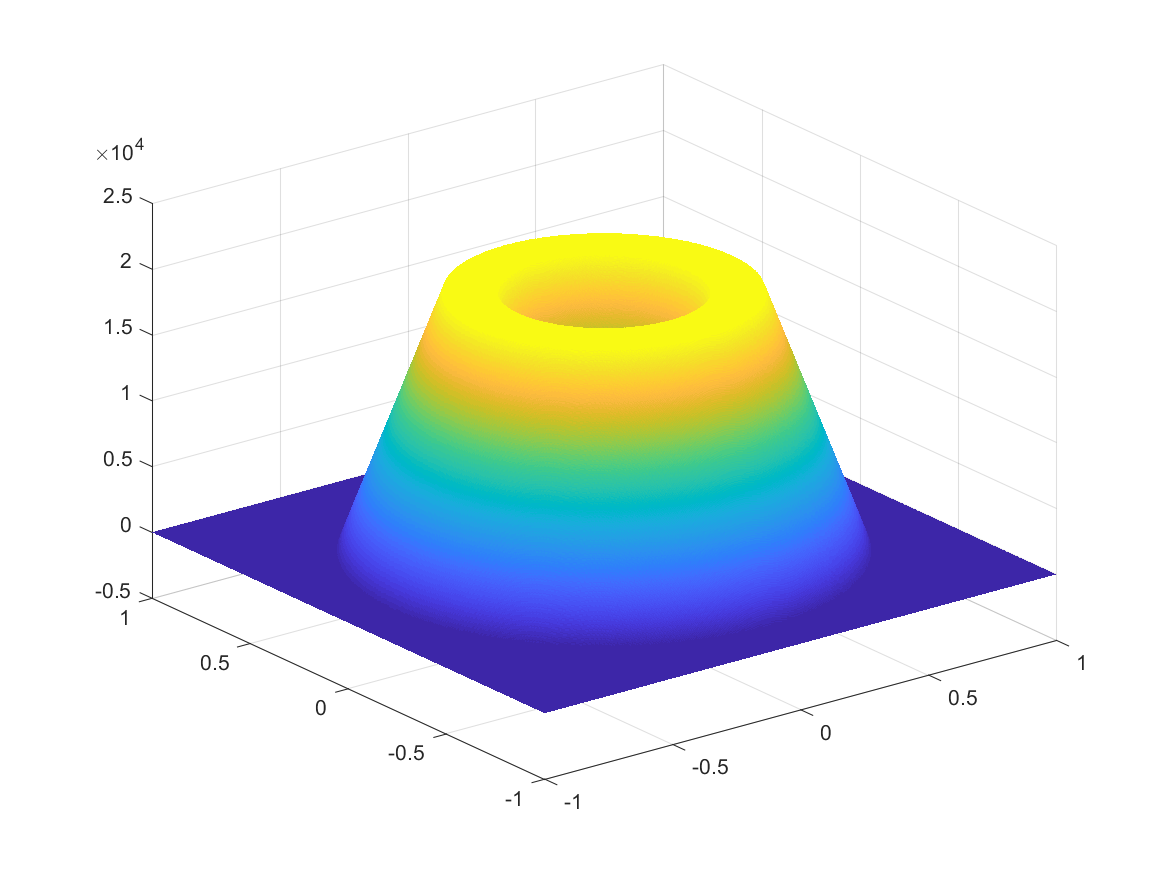
\includegraphics[trim = 40 30 30 30, clip, width=\linewidth]
      {pictures/chapExperiments/secGeneralInfo/f01Plots/inSi1e4.png}
    \label{fig:f01AlphaLargeInSi}
  \end{subfigure}
  \quad
  \begin{subfigure}[b]{.48\linewidth}
    \centering
    \caption{$f_{10^4}$ entlang der x- und y-Achse}
    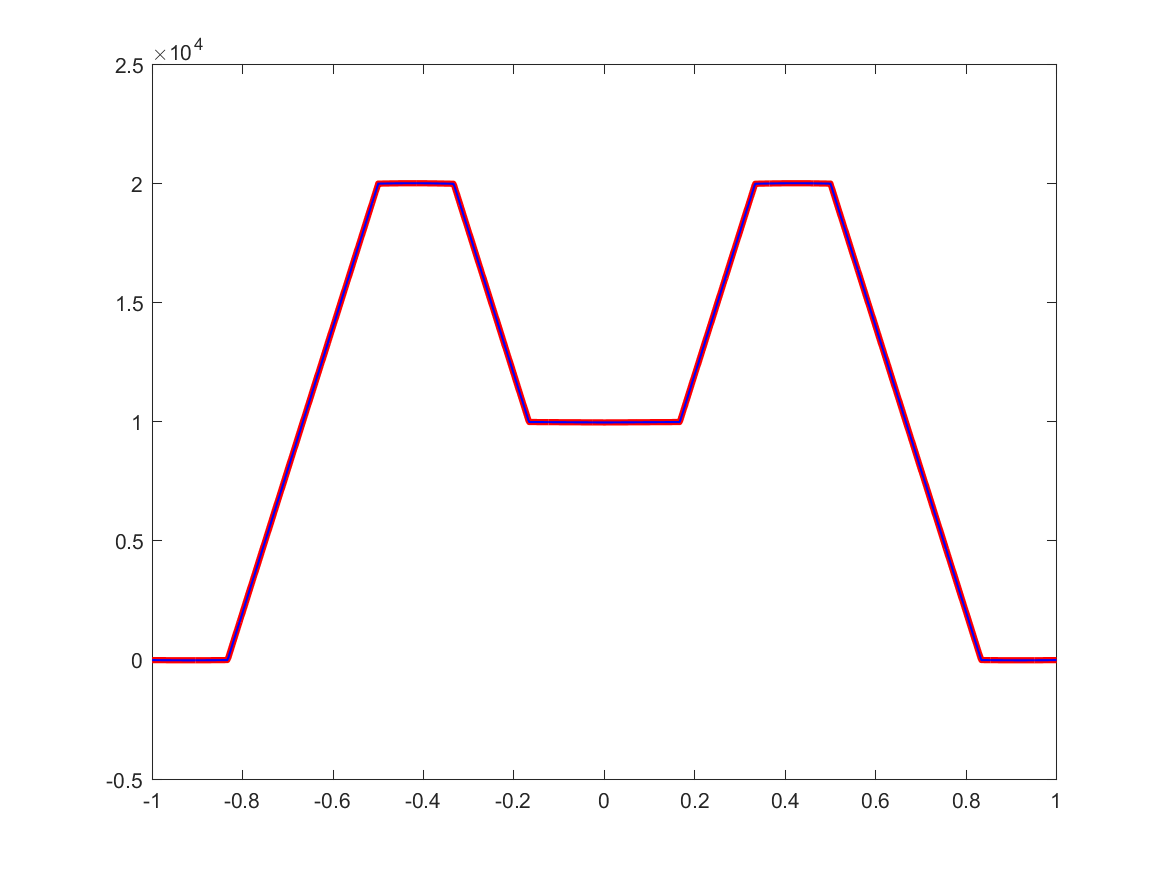
\includegraphics[trim = 50 30 50 20, clip, width=\linewidth]
      {pictures/chapExperiments/secGeneralInfo/f01Plots/inSi1e4Axis.png}
    \label{fig:f01AlphaLargeInSiAxis}
  \end{subfigure}

  \begin{subfigure}[b]{.48\linewidth}
    \centering
    \caption{$u$}
    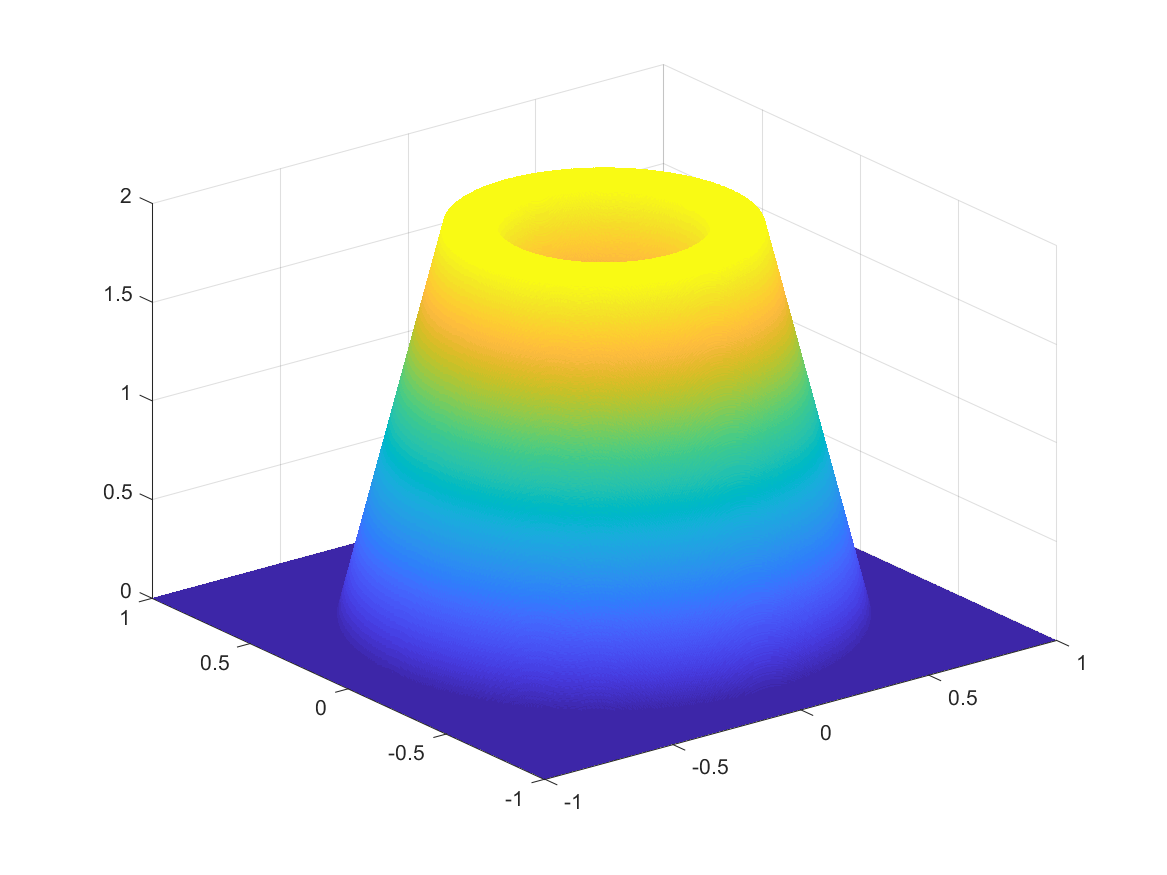
\includegraphics[trim = 40 30 30 30, clip, width=\linewidth]
      {pictures/chapExperiments/secGeneralInfo/f01Plots/exactSolution.png}
    \label{fig:f01ExactSol}
  \end{subfigure}
  \quad
  \begin{subfigure}[b]{.48\linewidth}
    \centering
    \caption{$u$ entlang der x- und y-Achse}
    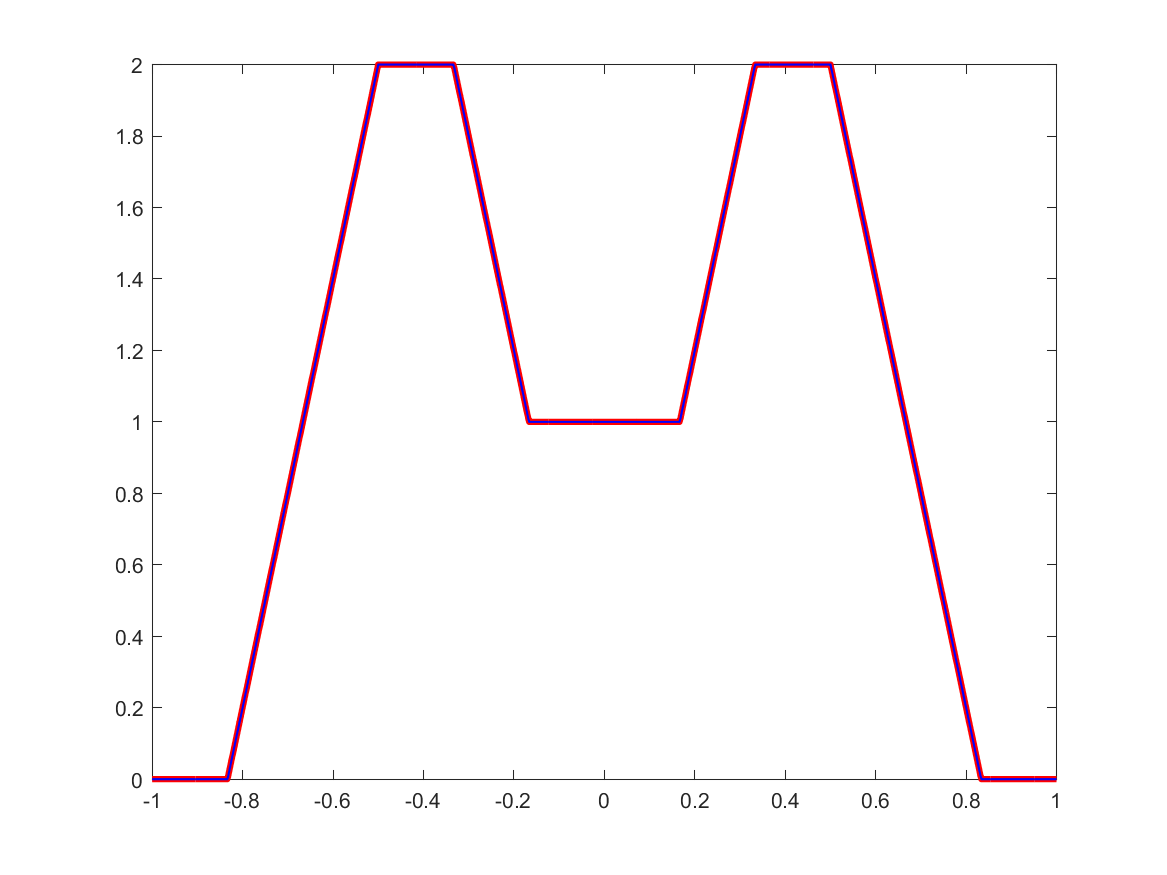
\includegraphics[trim = 50 30 50 20, clip, width=\linewidth]
      {pictures/chapExperiments/secGeneralInfo/f01Plots/exactSolutionAxis.png}
    \label{fig:f01ExactSolAxis}
  \end{subfigure} 
  \caption{Funktionen $f_\alpha$ und $u$ sowie deren
  Darstellungen entlang der x-Achse (blau) und der y-Achse (rot) für
  $\alpha\in\{1,10^4\}$}
  \label{fig:f01Plots}
\end{figure}
Die schwachen Gradienten von $u$ und $f_\alpha$ können bestimmt werden mithilfe
der partiellen Ableitungen
\begin{align*}
  \partial_r f_\alpha(r)
  &=
  \begin{cases}
    108,
    & \text{falls } r\in\left[0,\frac{1}{6}\right]\!,\\
    6\alpha\beta(6r-1)^{\beta-1} +\frac{1}{r^2}, 
    & \text{falls } r\in\left(\frac{1}{6},\frac{1}{3}\right]\!,\\
    \left(36\pi^2+\frac{1}{r^2}\right)\cos(\pi(6r-2))
    + \frac{6\pi}{r}\sin(\pi(6r-2)), 
    & \text{falls } r\in\left(\frac{1}{3},\frac{1}{2}\right]\!,\\
    -\left(6\alpha\beta\left( \frac{5}{2}-3r \right)^{\beta-1}+
    \frac{1}{r^2}\right),
    & \text{falls } r\in\left(\frac{1}{2},\frac{5}{6}\right]\!,\\
    -\left( \left( 18\pi^2+\frac{1}{2r^2} \right)\cos(\pi(6r-5))
    +\frac{1}{2r^2} + \frac{3\pi}{r}\sin(\pi(6r-5))\right)\!, 
    &\text{falls } r\in\left(\frac{5}{6},\infty\right)\!,
  \end{cases}
\end{align*}
und 
\begin{align*}
  \partial_r u(r) 
  &= 
  \begin{cases}
    0,
    & \text{falls } r\in\left[0,\frac{1}{6}\right]\!,\\
    6\beta(6r-1)^{\beta-1}, 
    & \text{falls } r\in\left(\frac{1}{6},\frac{1}{3}\right]\!,\\
    0, 
    & \text{falls } r\in\left(\frac{1}{3},\frac{1}{2}\right]\!,\\
    -6\beta\left( \frac{5}{2}-3r \right)^{\beta-1},
    & \text{falls } r\in\left(\frac{1}{2},\frac{5}{6}\right]\!,\\
    0,
    &\text{falls } r\in\left(\frac{5}{6},\infty\right)\!.
  \end{cases}
\end{align*} 
Durch Kenntnis des schwachen Gradienten von $u$ erhalten wir für das Experiment
mit Eingangssignal $f_\alpha$ die Approximation $E(u)\approx -2.05803$ für
$\alpha=1$ und $E(u)\approx -20\,580.34076$ für $\alpha=10^4$.
Ein weiteres Eingangssignal, welches wir in mehreren der folgenden Abschnitte
nutzen werden, ist das Graufarbenbild \texttt{cameraman} aus
\cref{fig:cameraman}, aus dem nach \Cref{rem:grayscalePictureInputSignal} ein
\texttt{function\_handle} erzeugt wird.


\section{Wahl der Parameter für die primale-duale Iteration}
\label{sec:choiceOfParameters}

Zunächst interessiert uns, wie der Parameter $\tau$ aus
\Cref{alg:primalDualIteration} gewählt werden sollte.
Durch \Cref{thm:convergenceIteration} ist uns bereits bekannt, dass
wir die Konvergenz der primalen-dualen Iteration nach ebendiesem Theorem nur 
für $\tau\in (0,1]$ garantieren können.
\begin{figure}[p]
  \centering
  \begin{subfigure}[b]{.48\linewidth}
    \caption{Eingangssignal $f_1$}
    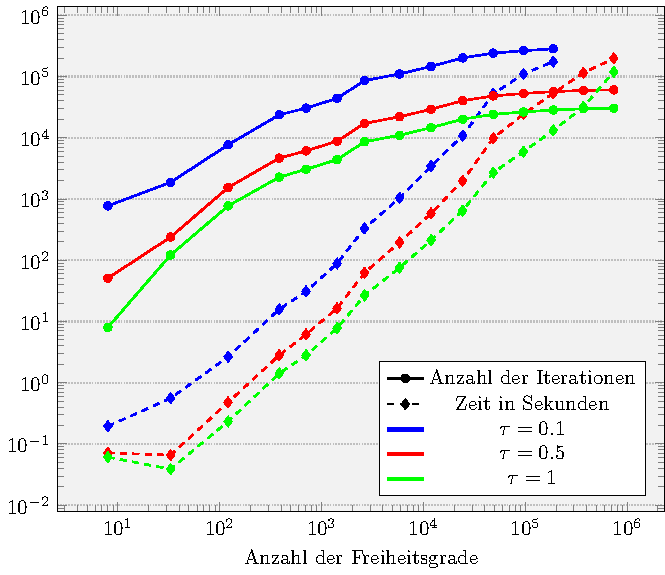
\includegraphics[width=\linewidth]
      {pictures/chapExperiments/secParameters/parTau/f01/miscF.pdf}
    \label{fig:parTauMiscF}
  \end{subfigure}
  \quad
  \begin{subfigure}[b]{.48\linewidth}
    \centering
    \caption{Eingangssignal \texttt{cameraman}}
    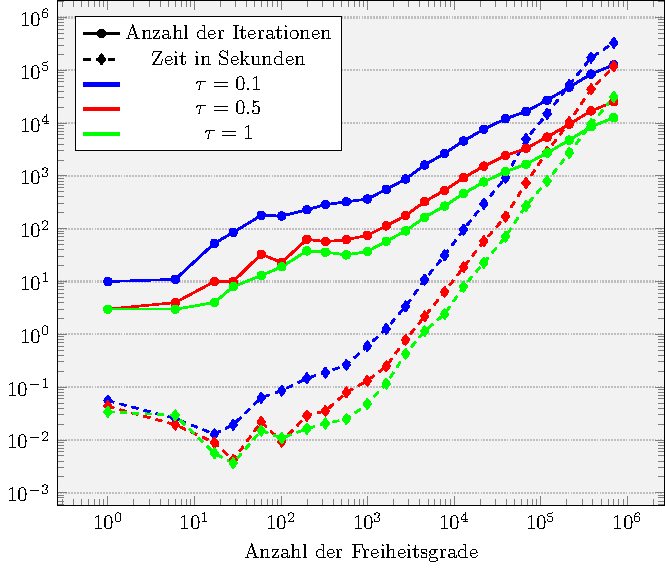
\includegraphics[width=\linewidth]
      {pictures/chapExperiments/secParameters/parTau/cam/miscCam.pdf}
    \label{fig:parTauMiscCam}
  \end{subfigure}
  \caption{Anzahl der Iterationen und benötigte Zeit für die primalen-dualen
    Iterationen während des AFEM-Algorithmus mit verschiedenen Werten von
    $\tau$ für die Eingangssignale $f_1$ und \texttt{cameraman}} 
  \label{fig:parTauMisc}
\end{figure}
In \Cref{fig:parTauMisc} sehen wir, dass die Anzahlen der Iterationsschritte,
und damit auch die Laufzeiten, der primalen-dualen Iterationen während der
AFEM-Routine umso größer sind, je kleiner $\tau$ gewählt wird.
\begin{figure}[p]
  \centering
  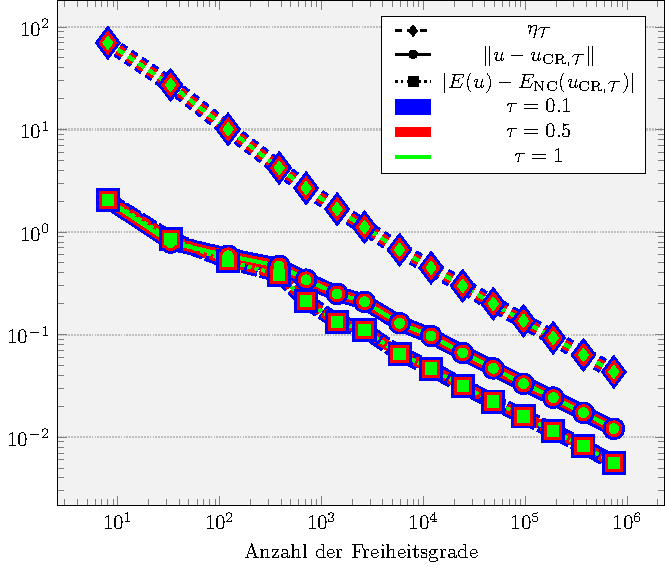
\includegraphics[width=.8\linewidth]
    {pictures/chapExperiments/secParameters/parTau/f01/convergenceF.pdf}
  \caption{Ergebnisse des Programms mit verschieden Werten von $\tau$ für das
    Eingangssignal $f_1$}
  \label{fig:parTauConvergence}
\end{figure}
Da sich die betrachteten Graphen in \Cref{fig:parTauConvergence} für die
verschiedenen Wahlen von $\tau$ nicht sichtbar unterscheiden, vermuten wir,
dass die ideale Wahl für $\tau$ die maximale nach
\Cref{thm:convergenceIteration} zulässige ist.
Deshalb wählen wir für unsere Experimente $\tau=1$.
Eine mögliche Erklärung für unsere Beobachtung liefert der Beweis von
\Cref{thm:convergenceIteration}.
Die darin bewiesene Ungleichung \eqref{eq:upperBoundIterationError} impliziert
\begin{align}
  \label{eq:nrIterationsInequality}
  \sum_{j=1}^\infty\Vert \ucrt - \ujt \Vert^2 
  \leq
  \frac{1}{2\alpha\tau}
  \left(\vvvert \ucrt - u_{0,\Tcal}\vvvert^2_\nc 
  + \left\Vert \bar\Lambda_{0,\Tcal} - \Lambda_{0,\Tcal}\right\Vert^2\right)\!. 
\end{align}
Die rechte Seite ist antiproportional zu $\tau$, womit womöglich
die Folge $(\left\Vert \ucr - \ujt\right\Vert)_{j\in\Nbb}$ schneller gegen $0$
konvergiert und damit auch das Abbruchkriterium \eqref{eq:terminationCriterion}
nach einer geringeren Anzahl von Iterationen erfüllt ist. 
Allerdings schließt der Beweis von \Cref{thm:convergenceIteration} die
Konvergenz der primalen-dualen Iteration für $\tau>1$ nicht aus.
\begin{figure}[p]
  \centering
  \begin{subfigure}[b]{.48\linewidth}
    \centering
    \caption{Messungen der Updates}
    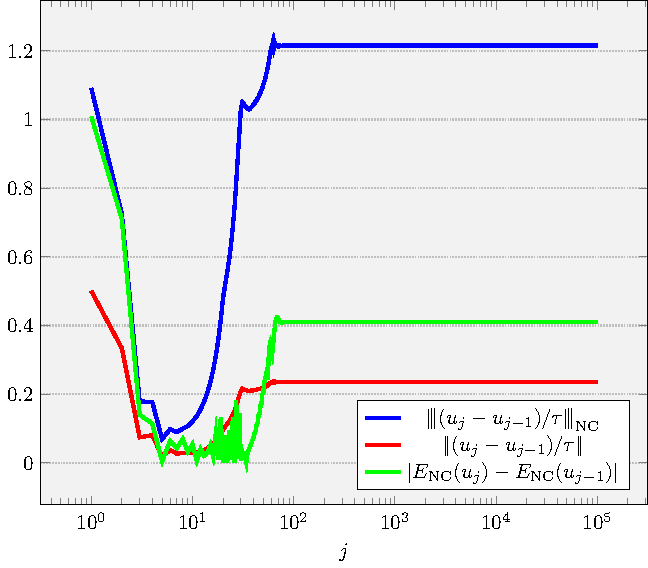
\includegraphics[width=\linewidth]
      {pictures/chapExperiments/secParameters/parTau/f01NoConv/1Dot2/convIter.pdf}
    \label{fig:parTauNoConvergenceUpdates}
  \end{subfigure}
  \quad
  \begin{subfigure}[b]{.47\linewidth}
    \centering
    \caption{Nichtkonforme Energien}
    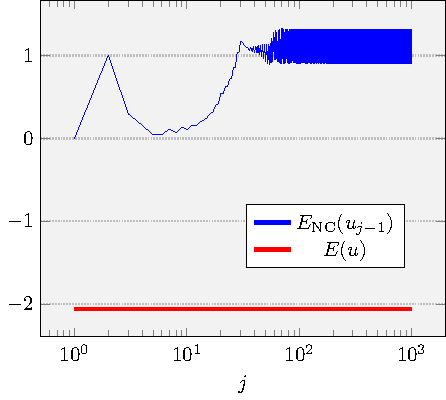
\includegraphics[width=\linewidth]
      {pictures/chapExperiments/secParameters/parTau/f01NoConv/1Dot2/convEnergy.pdf}
    \label{fig:parTauNoConvergenceEnergy}
  \end{subfigure}
  \caption{Verschiedene Messungen der Updates (a) und Verlauf der nichtkonformen
    Energien der ersten $1000$ Iterate (b) der primalen-dualen Iteration auf
    der Triangulierung \texttt{BigSquare} aus \Cref{fig:triangBigSquare} mit
    $\tau=1.2$ für das Eingangssignal $f_1$}
  \label{fig:parTauNoConvergence}
\end{figure}
Wie aber in \Cref{fig:parTauNoConvergence} zu sehen, haben wir schon für
$\tau=1.2$ ein Beispiel gefunden, bei dem nicht davon ausgegangen werden kann,
dass die primale-duale Iteration konvergiert.
Dabei wurde die Iteration nach $10^5$ Schritten abgebrochen, da kein anderes
Verhalten mehr zu erwarten war.
Zusätzlich legitimiert wird der Abbruch nach $10^5$ Iterationen dadurch, dass
in \Cref{fig:parTauMiscF} auf der gleichen Triangulierung für die
suboptimale Wahl $\tau = 0.1$ weniger als $10^3$ Iterationen und für die Wahl
$\tau=1$ sogar weniger als $10$ Iterationen benötigt wurden.
Weiterhin zeigt \Cref{fig:parTauNoConvergenceUpdates}, dass auch für andere
Varianten, den Unterschied zweier aufeinanderfolgender Iterate im
Abbruchkriterium \eqref{eq:terminationCriterion} zu messen, die Iteration in
der Regel nicht abbricht.
Es scheint nach \Cref{fig:parTauNoConvergenceEnergy} außerdem festzustehen,
dass die nichtkonformen Energien der Iterate nach etwa $100$ Iterationen
oszillierend Werte annehmen.
Somit bleibt insgesamt festzuhalten, dass eine Konvergenzaussage im Wortlaut
von \Cref{thm:convergenceIteration} für $\tau\in(0,1.2]$ nicht mehr bewiesen
werden kann.

Als Nächstes begründen wir die Wahl $\epsstop = 10^{-4}$ für das
Abbruchkriterium \eqref{eq:terminationCriterion}.
\begin{figure}[p]
  \centering
  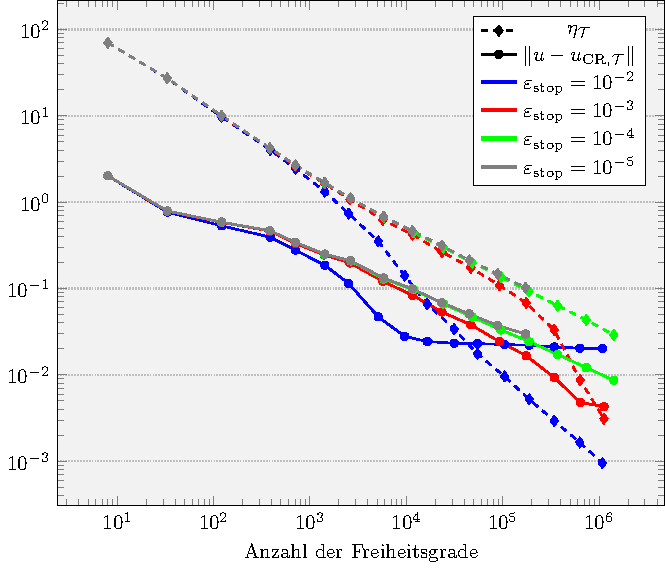
\includegraphics[width=.8\linewidth]
    {pictures/chapExperiments/secParameters/parEpsStop/f01/convergenceF.pdf}
  \caption{Ergebnisse des Programms mit verschieden Werten von $\epsstop$ für
    das Eingangssignal $f_1$}
  \label{fig:parEpsStopConvergence}
\end{figure}
Wie in \Cref{fig:parEpsStopConvergence} zu sehen, stagniert der exakte
$L^2$-Fehler für $\epsstop=10^{-2}$ ab circa $10^4$ Freiheitsgraden und es
lässt sich erahnen, dass dieser Effekt auch für $\epsstop=10^{-3}$ ab ungefähr
$6\cdot 10^5$ Freiheitsgraden einsetzt.  
Dabei ist der erreichte Fehler für $\epsstop=10^{-3}$ geringer als
für $\epsstop=10^{-2}$.
Da für $\epsstop\in\{10^{-5},10^{-4}\}$ bis $10^6$ Freiheitsgrade dieses
Verhalten noch nicht zu sehen ist, scheint dies an einem zu frühen Abbruch der
Iteration durch eine zu große Wahl von $\epsstop$ zu liegen. 
Bei einer hohen Anzahl an Freiheitsgraden, das heißt bei kleinen Netzweiten,
muss also $\epsstop$ ausreichend klein sein, um die beobachtete Stagnation
des exakten Fehlers zu verhindern.
Da wir bei den Experimenten in dieser Arbeit $10^6$ Freiheitsgrade nicht
deutlich überschreiten und sich bis dahin die Ergebnisse für die Wahlen
$10^{-4}$ und $10^{-5}$ für $\epsstop$ in \Cref{fig:parEpsStopConvergence} kaum
unterscheiden, die Wahl $\epsstop=10^{-5}$ aber eine wesentlich längere
Laufzeit des Programms verursacht, begründen wir damit unsere Wahl
$\epsstop=10^{-4}$.
Allerdings bleibt anzumerken, dass der Verfeinerungsindikator $\etaT$ für alle
getesteten Wahlen von $\epsstop$ weiter fällt. 
Um dies zu untersuchen, betrachten wir die \Cref{def:refinementIndicator} von
$\etaT$.
Aus dieser folgt
\begin{align}
  \label{eq:etaEstimate}
  \etaT 
  \leq
  \max_{T\in\Tcal}|T|\Vert f-\alpha\ucrt\Vert^2
  + 2\max_{T\in\Tcal}|T|^{\gamma/2}\sum_{F\in\Ecal}\Vert[\ucrt]_F\Vert_{L^1(F)}.
\end{align}
Stagniert während der AFEM-Routine $\Vert u-\ucrt\Vert$, ist in Anbetracht
der Interpretation des ROF-Modells aus \Cref{chap:introduction} nicht
ausschließbar, dass $\Vert f-\alpha\ucrt\Vert^2$ ebenfalls stagniert.
Außerdem können wir nach den Überlegungen zu \Cref{fig:f01JumpTerms} in
\Cref{sec:experimentsWithExactSolution} davon ausgehen,
dass wahrscheinlich auch in den Experimenten aus
\Cref{fig:parEpsStopConvergence} die Terme
$\sum_{F\in\Ecal}\Vert[\ucrt]_F\Vert_{L^1(F)}$ im Verlauf des AFEM-Algorithmus
nicht gegen $0$ konvergieren.
Dennoch ist nach Ungleichung \eqref{eq:etaEstimate} die Konvergenz von $\etaT$
gegen $0$ weiterhin möglich, solange die Flächen der Dreiecke $T\in\Tcal$
reduziert werden.  
Insbesondere kann davon ausgegangen werden, dass, nach Eintreten der 
beschriebenen Stagnation, der Flächeninhalt von Dreiecken beim Markieren durch 
$\etaT$ zunehmend wichtiger wird.
\begin{figure}[p]
  \centering
  \begin{subfigure}[b]{.48\linewidth}
    \centering
    \caption{$\epsstop=10^{-2}$}
    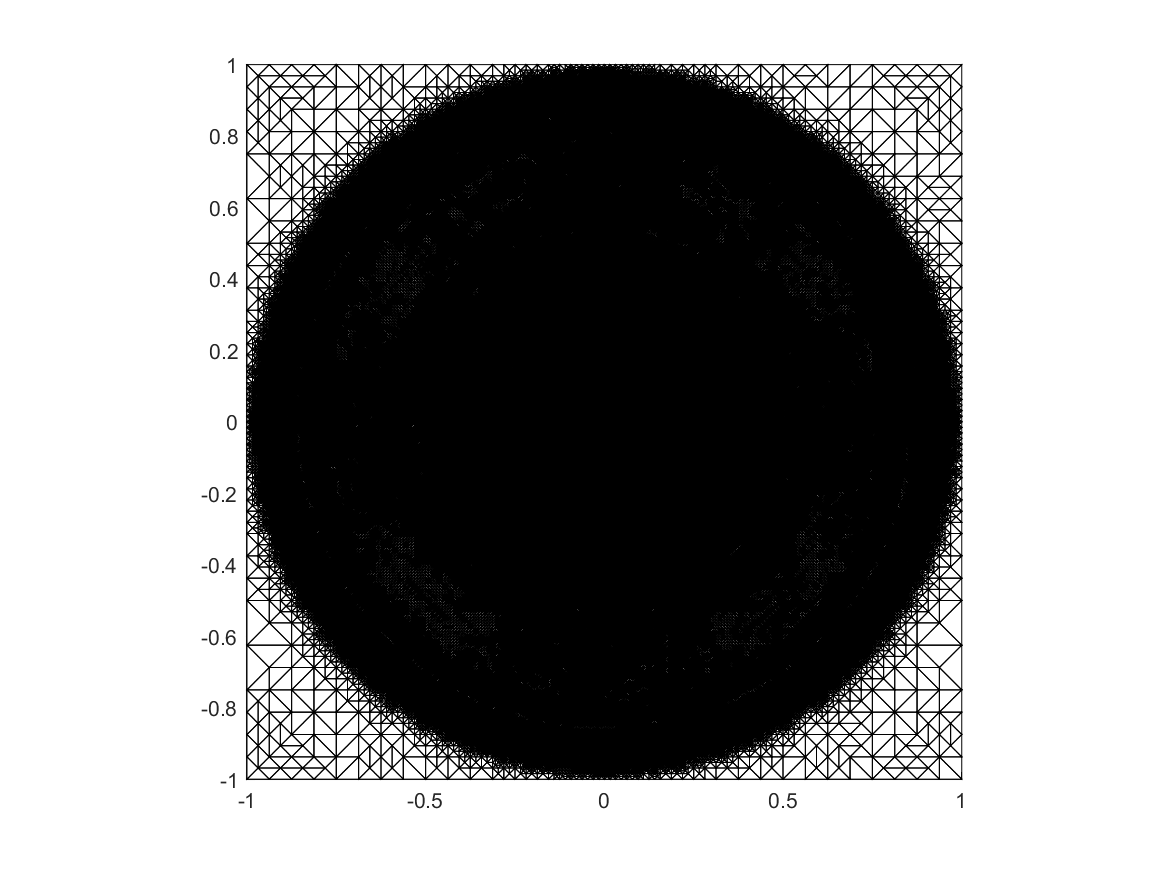
\includegraphics[trim = 100 30 80 20, clip, width=\linewidth]
      {pictures/chapExperiments/secParameters/parEpsStop/f01/1eM2/lvl15/triangulation.png}
    \label{fig:triangEpsStop1em2}
  \end{subfigure}
  \quad
  \begin{subfigure}[b]{.48\linewidth}
    \centering
    \caption{$\epsstop=10^{-5}$}
    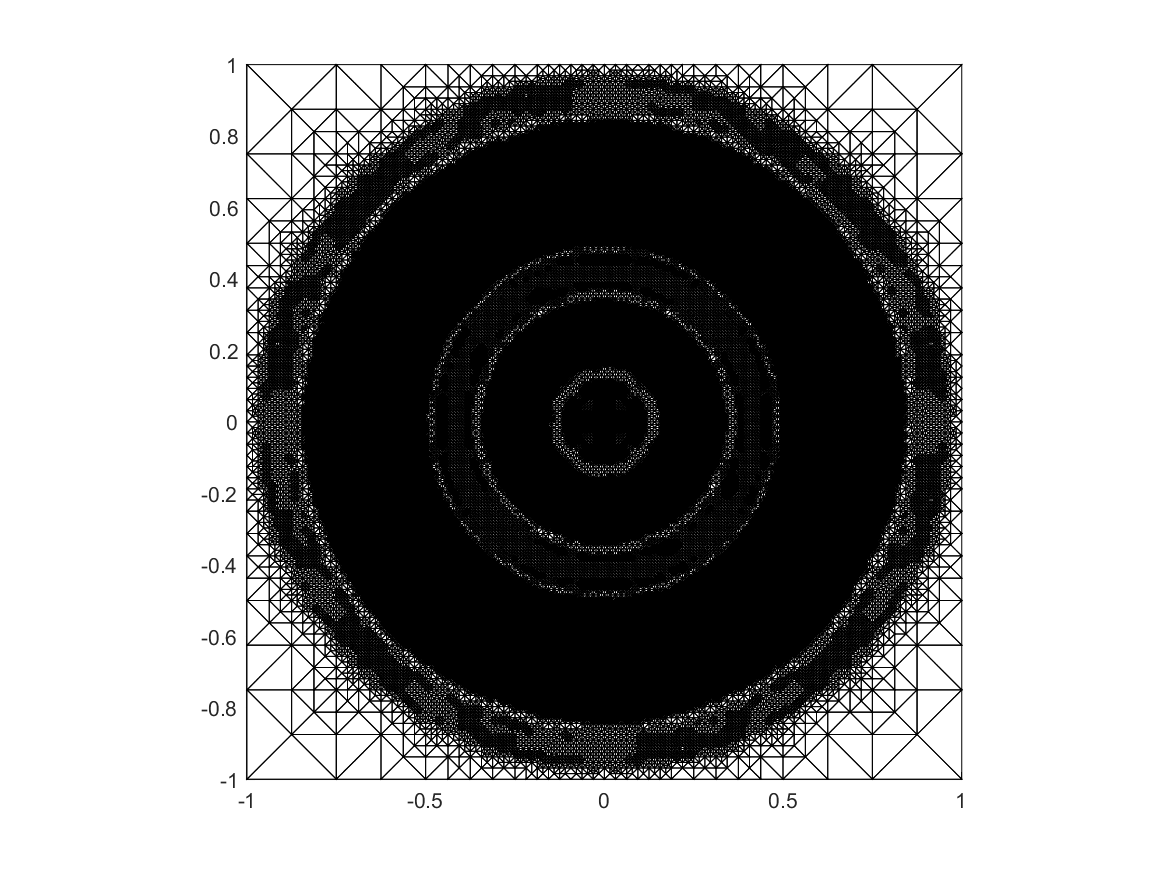
\includegraphics[trim = 100 30 80 20, clip, width=\linewidth]
      {pictures/chapExperiments/secParameters/parEpsStop/f01/1eM5/lvl14/triangulation.png}
    \label{fig:triangEpsStop1em5}
  \end{subfigure}
  \caption{Triangulierungen nach den Rechnungen mit verschiedenen Werten von
    $\epsstop$ nach jeweils circa 620\,000 Freiheitsgraden für das
    Eingangssignal $f_1$}
  \label{fig:triangEpsStop}
\end{figure}
Diese Vermutung scheint von \Cref{fig:triangEpsStop} gestützt zu werden, in der
wir sehen, dass bei einer vergleichbaren Anzahl von Freiheitsgraden der
abgebildeten Triangulierungen die Fläche des größten Dreiecks in
\Cref{fig:triangEpsStop1em2} zu $\epsstop=10^{-2}$ kleiner ist als die des
größten Dreiecks in \Cref{fig:triangEpsStop1em5} zu $\epsstop=10^{-5}$. 
Die vor Eintreten der Stagnation für $\epsstop\in\{10^{-3},10^{-2}\}$ im
Vergleich zu $\epsstop\in\{10^{-5},10^{-4}\}$ größere
Konvergenzgeschwindigkeit, die in \Cref{fig:parEpsStopConvergence} zu sehen
ist, lässt die Annahme zu, dass die Verfeinerung von Dreiecken mit großer
Fläche kurzzeitig eine effektive Strategie ist, insgesamt aber nicht zu
geringeren exakten Fehlern führt.


\section{Eigenschaften der primalen-dualen Iteration}
\label{sec:experimentsPrimalDualIteration}

Nun möchten wir anhand einiger Experimente mit Eingangssignal $f_1$ 
die primale-duale Iteration untersuchen.
\begin{figure}[p]
  \centering
  \begin{subfigure}[b]{.5\linewidth}
    \centering
    \caption{Nichtkonforme Energien der Iterate}
    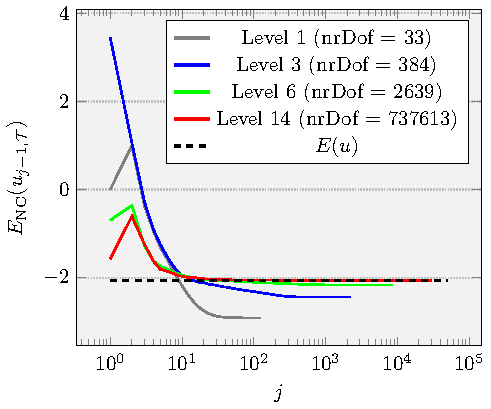
\includegraphics[width=\linewidth]
      {pictures/chapExperiments/secIterProps/lvlWise/convEnergy.pdf}
    \label{fig:iterationEnergyLevel}
  \end{subfigure}
  \quad
  \begin{subfigure}[b]{.46\linewidth}
    \centering
    \caption{Oszillierendes Beispiel}
    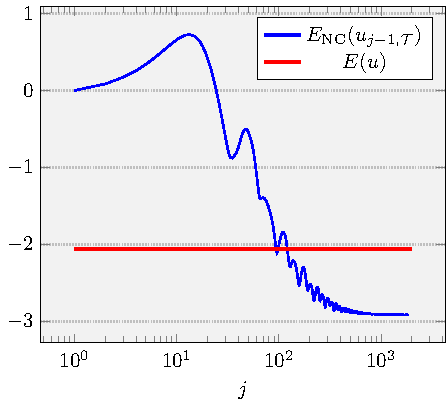
\includegraphics[width=\linewidth]
      {pictures/chapExperiments/secIterProps/osc/convEnergy.pdf}
    \label{fig:iterationEnergyOscillations}
  \end{subfigure}
  \caption{Entwicklung der nichtkonformen Energien der Iterate während der
    pri\-malen\--dualen Iteration auf verschiedenen Leveln der AFEM-Routine mit
    $\tau=1$ (a) und für ein Level mit 33 Freiheitsgraden und $\tau=10^{-1}$
    (b) für das Eingangssignal $f_1$}
  \label{fig:iterationEnergy}
\end{figure}
In \Cref{fig:iterationEnergyLevel} sehen wir an einer Auswahl von Leveln der
AFEM-Routine, dass die
nichtkonforme Energie $\Enc(\bullet)$ der Iterate von oben konvergiert. 
Dabei nimmt der Abstand des jeweiligen Grenzwerts zu der Energie der exakten
Lösung $E(u)$ mit zunehmender Anzahl von Freiheitsgraden ab.
Anhand des Ansteigens der nichtkonformen Energie im ersten Iterationsschritt
aller in \Cref{fig:iterationEnergyLevel} dargestellten Level, mit Ausnahme von
Level 3, ist aber auch klar erkennbar, dass die nichtkonformen Energien der
Iterate nicht monoton fallend konvergieren.
Dies können wir ebenfalls in \Cref{fig:iterationEnergyOscillations} sehen, in
der, auf einem Level mit 33 Freiheitsgraden für das gleiche Experiment mit
$\tau=10^{-1}$, die nichtkonformen Energien der Iterate oszillierend fallen.
Ebendieses Verhalten könnte ein Grund dafür sein, dass die  bis zum Abbruch der
primalen-dualen Iteration benötigte Anzahl an Iterationen für $\tau=10^{-1}$
deutlich höher ist als für $\tau=1$, wie wir bereits in \Cref{fig:parTauMiscF}
gesehen haben.
\begin{figure}[p]
  \centering
  \begin{subfigure}[b]{.5\linewidth}
    \centering
    \caption{Messungen der Updates}
    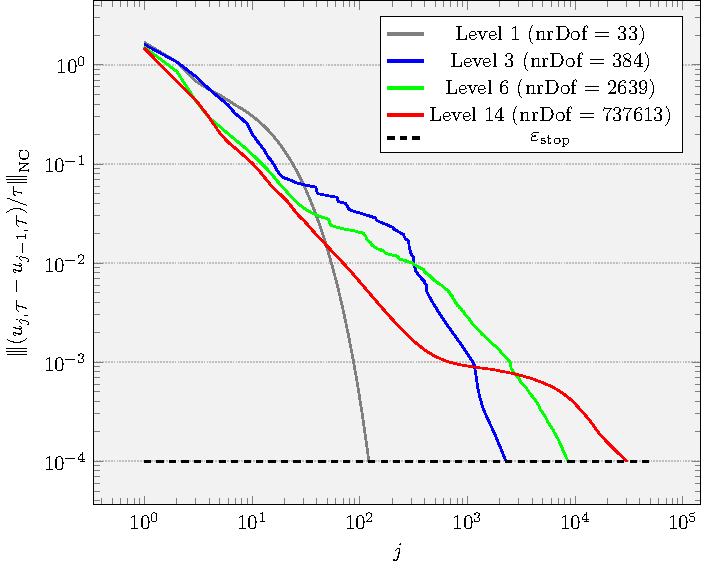
\includegraphics[width=\linewidth]
      {pictures/chapExperiments/secIterProps/lvlWise/termLvl.pdf}
    \label{fig:iterationLevel}
  \end{subfigure}
  \quad
  \begin{subfigure}[b]{.46\linewidth}
    \centering
    \caption{Varianten für die Messungen der Updates }
    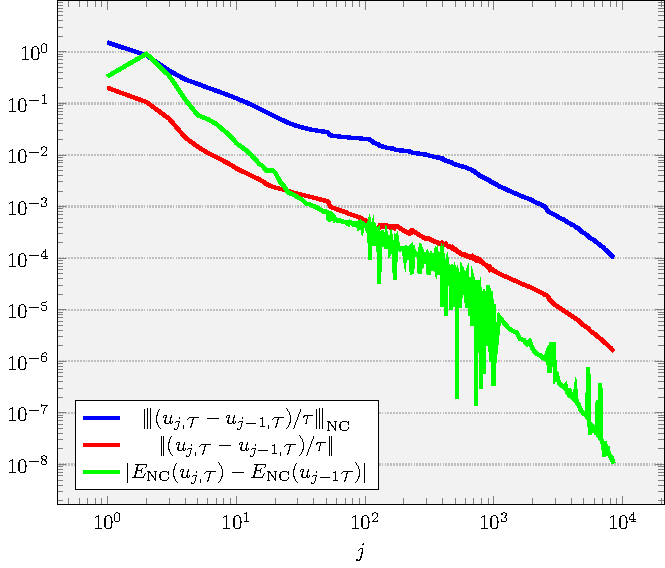
\includegraphics[width=\linewidth]
      {pictures/chapExperiments/secIterProps/lvlWise/termComp.pdf}
    \label{fig:iterationTerminationVariants}
  \end{subfigure}
  \caption{Verlauf der Messungen der Updates aus dem Abbruchkriterium 
    \eqref{eq:terminationCriterion} während der primalen-dualen Iteration auf
    verschiedenen Leveln der AFEM-Routine (a) und Verlauf von Varianten, diese
    Updates zu messen, für ein Level mit 2\,639 Freiheitsgraden (b) für das
    Eingangssignal $f_1$}
  \label{fig:iterationTermination}
\end{figure}
Als Nächstes betrachten wir \Cref{fig:iterationLevel}, in der die Entwicklung
der Messung des Unterschieds zweier aufeinanderfolgender Iterate im
Abbruchkriterium \eqref{eq:terminationCriterion} für verschiedene Level 
während der AFEM-Routine zu sehen ist.
Diese nimmt stets ohne Auffälligkeiten ab, bis sie den Wert $\epsstop$
erreicht.
Dabei ist wieder zu erkennen, dass die Anzahl der dazu benötigten Iterationen
mit steigender Anzahl an Freiheitsgraden zunimmt.
Zusätzlich sind in \Cref{fig:iterationTerminationVariants} für das sechste Level
derselben Rechnung die Verläufe zweier weiterer Varianten, 
den Unterschied von zwei aufeinanderfolgenden Iteraten zu messen, zu sehen.
Deren Konvergenz gegen $0$ ist zu erwarten, weshalb sie ebenfalls für das
Abbruchkriterium in Betracht gezogen werden könnten.
Dabei unterscheidet sich die Variante, bei der lediglich die $L^2$-Norm
anstelle der Energienorm verwendet wird, nur um einen Faktor von etwa
$10^2$ von der im Programm benutzten. 
Dies passt zur bekannten Theorie, da die Norm $\vvvert\bullet\vvvert_\NC$
ungefähr so skaliert wie $h^{-1}\Vert\bullet\Vert$ (cf. \cite[Lemma 3.5, Lemma
3.7]{Bar15}), wobei für das in \Cref{fig:iterationTerminationVariants} gezeigte
Level ungefähr gilt $h\approx 10^{-2}$.
Dementsprechend ist davon auszugehen, dass bei Wahl dieses Abbruchkriteriums 
nur die Toleranz $\epsstop$ angepasst werden müsste.
Die andere Variante zum Messen des Updates, das heißt der Betrag der Differenz
der nichtkonformen Energien zweier Iterate, scheint sich aber,
aufgrund der auftretenden Oszillationen, nur schlecht für ein 
Abbruchkriterium zu eignen.
Abschließend können wir festhalten, dass sich demnach das von uns gewählte 
Abbruchkriterium \eqref{eq:terminationCriterion} als sinnvoll erwiesen hat.

\vfill

\section{Experimente mit bekannter exakter Lösung}
\label{sec:experimentsWithExactSolution}

In diesem Abschnitt möchten wir zunächst die Ergebnisse der Experimente mit
Eingangssignal $f_1$ bei adaptiver und uniformer Netzverfeinerung untersuchen
und einige Aussagen aus den theoretischen Kapiteln dieser Arbeit validieren.
\begin{figure}[p]
  \DTLloaddb{db}{data/currentDataReducedStandardF01LvlFinal.csv}
  \DTLassign{db}{1}{\nrDof=nrDof} 
  \DTLgdeletedb{db}
  \centering
  \begin{subfigure}[b]{.48\linewidth}
    \centering
    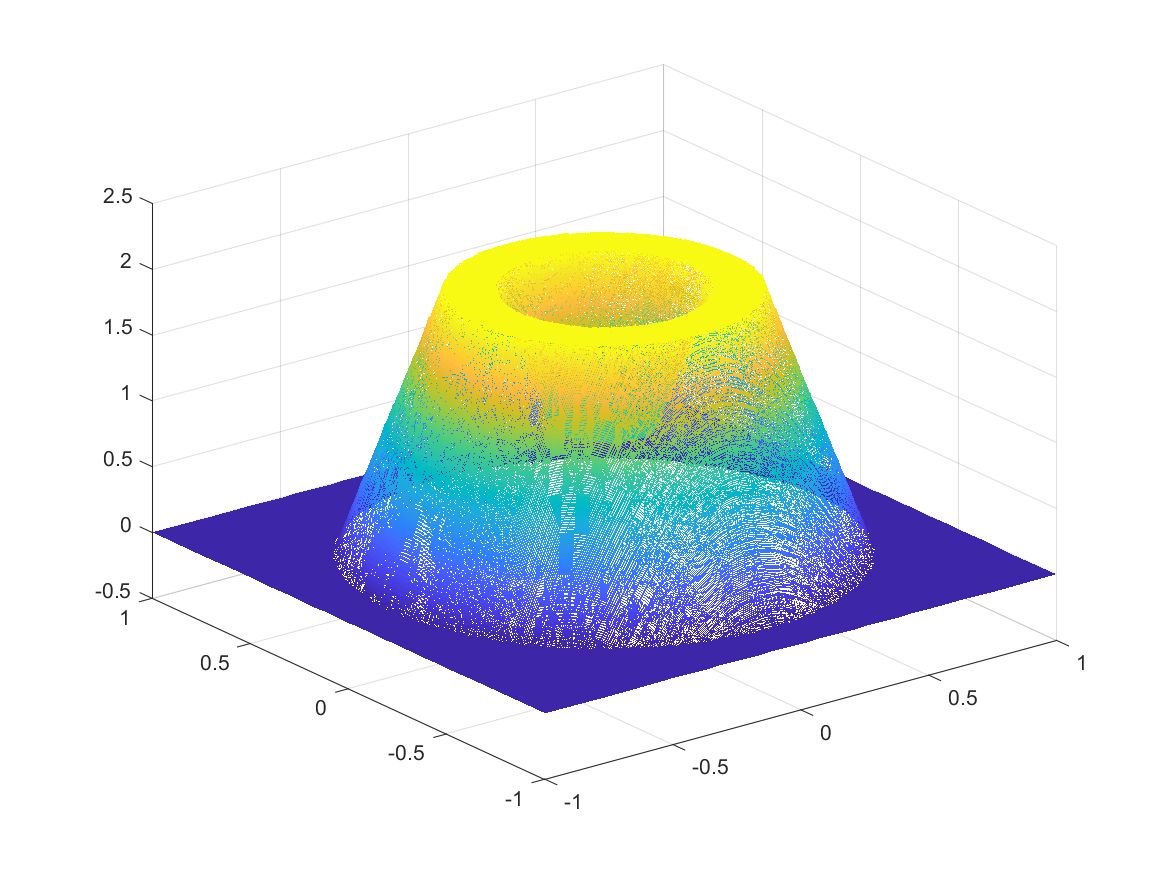
\includegraphics[trim = 40 30 30 30, clip, width=\linewidth]
      {pictures/chapExperiments/secExactSol/f01/adaptive/lvl14/solution.png}
    \label{fig:f01SolAdaptivePlot}
  \end{subfigure}
  \quad
  \begin{subfigure}[b]{.48\linewidth}
    \centering
    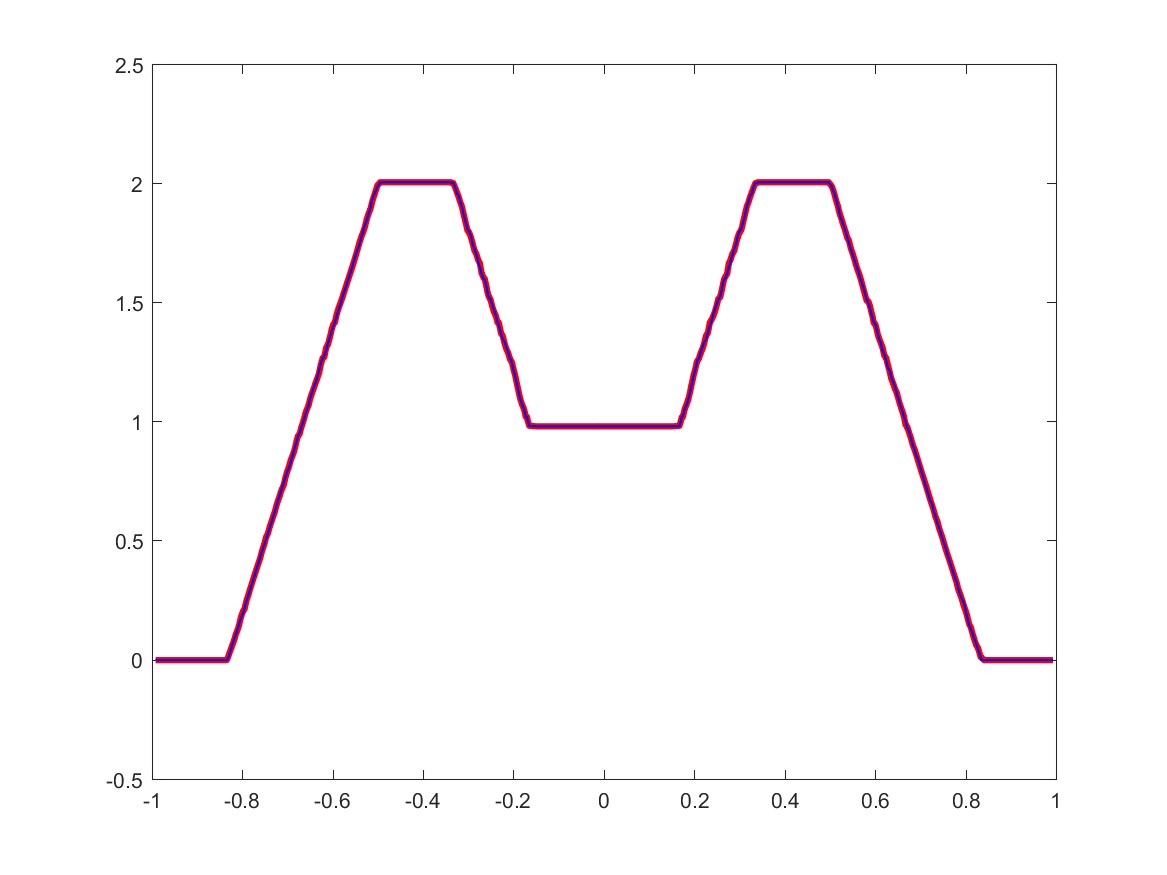
\includegraphics[trim = 50 30 50 20, clip, width=\linewidth]
      {pictures/chapExperiments/secExactSol/f01/adaptive/lvl14/solutionAxis.png}
    \label{fig:f01SolAdaptiveAxis}
  \end{subfigure}
  \caption{Lösung der Rechnung bei adaptiver Netzverfeinerung sowie deren
  Darstellungen entlang der x-Achse (blau) und der y-Achse (rot) nach etwa
  740\,000 Freiheitsgraden mit Eingangssignal $f_1$ }
  \label{fig:f01SolAdaptive}
\end{figure}
Die Lösung des Experiments mit adaptiver Netzverfeinerung ist in
\Cref{fig:f01SolAdaptive} dargestellt und ähnelt erkennbar der exakten Lösung
$u$ aus \Cref{fig:f01Plots}.
\begin{figure}[p]
  \centering
  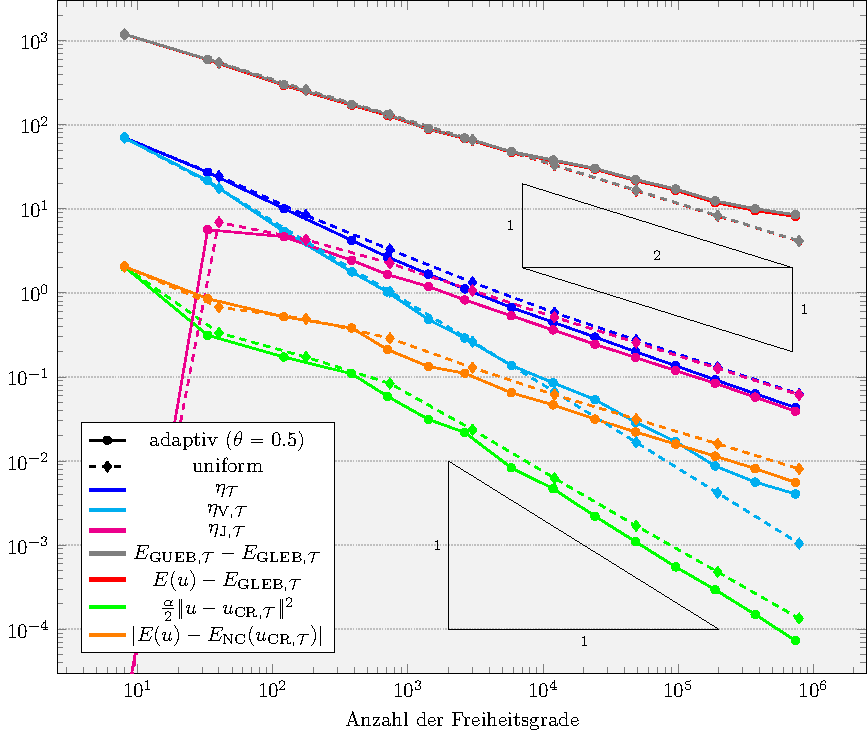
\includegraphics[width=.8\linewidth]
    {pictures/chapExperiments/secExactSol/f01/conv.pdf}
  \caption{Ergebnisse der Rechnungen mit adaptiver und uniformer 
    Netzverfeinerung für das Eingangssignal $f_1$}
  \label{fig:f01Convergence}
\end{figure}
Wie in \Cref{fig:f01Convergence} zu sehen, unterscheiden sich die
Konvergenzraten bei uniformer und adaptiver Netzverfeinerungen nur für den
Anteil $\etaV$ des Verfeinerungsindikators aus \Cref{def:refinementIndicator}
und für die Differenzen $\Egueb-\Egleb$ sowie $E(u)-\Egleb$ mit den
garantierten oberen und unteren Energieschranken $\Egueb$ und $\Egleb$ aus
\Cref{sec:refinementIndicatorAndGuaranteedBounds}.
Dabei können die Ratenunterschiede für diese Differenzen auf die für $\etaV$
zurückgeführt werden, denn nach Definition von $\Egleb$ in \Cref{eq:gleb}
und von $\etaV$ ist zu erwarten, dass der Wert von $\Egleb$ umso kleiner
ist, je größer der Wert von $\etaV$ ist. 
Tatsächlich nimmt in \Cref{fig:f01Convergence} bei adaptiver Netzverfeinerung 
$\etaV$ größere Werte an als bei uniformer, weshalb sich die beiden Graphen, in
denen $\Egleb$ subtrahiert wird, ebenso verhalten.
Die Konvergenzrate von $\etaV$ ist bei uniformer Netzverfeinerung etwa $1$ und
scheint bei adaptiver Netzverfeinerung kleiner als $1$ aber womöglich
größer als 1/2 zu sein.  
Allerdings wirken sich diese Ratenunterschiede von $\etaV$ bei adaptiver und
uniformer Netzverfeinerung nicht auf den Verfeinerungsindikator $\etaT$ aus,
denn dieser wird mit zunehmenden Freiheitsgraden deutlich von seinem Anteil
$\etaJ$ dominiert.
Damit hat $\etaT$, ebenso wie $\etaJ$, die Rate 1/2.

Durch \Cref{fig:iterationEnergyLevel} war bereits zu vermuten, dass die
nichtkonformen Energien der diskreten Lösungen $\Enc(\ucrt)$ gegen die Energie 
der exakten Lösung $E(u)$ konvergiert.
Nun sehen wir, dass $|E(u)-\Enc(\ucrt)|$ tatsächlich konvergiert mit einer 
Rate von etwa 1/2.
Weiterhin erwarten wir nach der Herleitung des diskreten Problems in
\Cref{sec:discreteProblemFormulation}, dass $E(\ucrt)$, im Gegensatz zu
$\Enc(\ucrt)$, nicht gegen $E(u)$ konvergiert.
\begin{figure}[p]
  \centering
  \begin{subfigure}[b]{.48\linewidth}
    \centering
    \caption{Entwicklung der Sprungterme}
    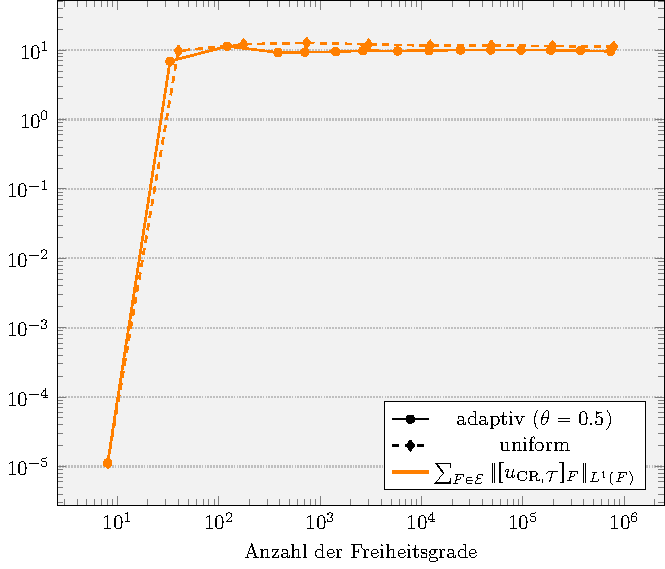
\includegraphics[width=\linewidth]
      {pictures/chapExperiments/secExactSol/f01/jumpTerms.pdf}
    \label{fig:f01JumpTerms}
  \end{subfigure}
  \quad
  \begin{subfigure}[b]{.48\linewidth}
    \centering
    \caption{Entwicklung der Energieschranken}
    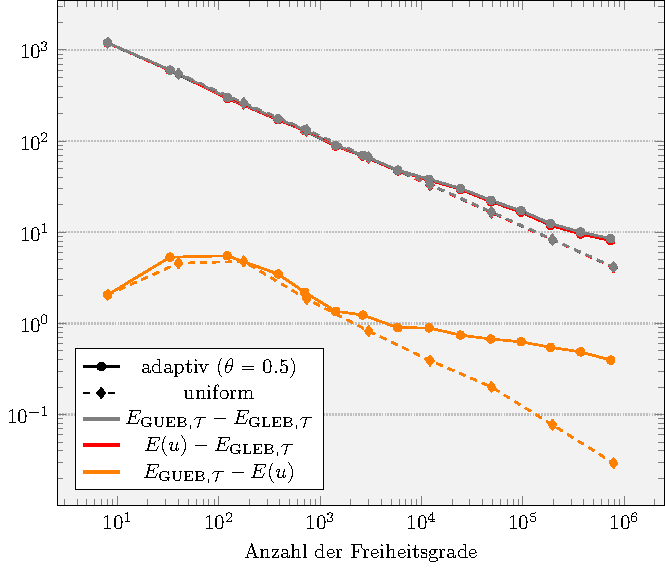
\includegraphics[width=\linewidth]
      {pictures/chapExperiments/secExactSol/f01/energyDiffs.pdf}
    \label{fig:f01DiffGuebExactE}
  \end{subfigure}
  \caption{Zusätzliche Ergebnisse der Rechnungen mit adaptiver und uniformer 
    Netzverfeinerung für das Eingangssignal $f_1$}
  \label{fig:f01SupplementaryInfo}
\end{figure}
Dies wird experimentell bestätigt durch \Cref{fig:f01JumpTerms}, in der wir
sehen, dass in unserer nichtkonformen Formulierung \Cref{prob:discreteProblem}
der Term $\sum_{F\in\Ecal}\Vert[\ucrt]_F\Vert_{L^1(F)}=E(\ucrt)-\Enc(\ucrt)$
tatsächlich nicht minimiert wird. 
Zwar sind die jeweiligen Sprünge zwischen zwei Dreiecken bei einer hohen Anzahl
von Freiheitsgraden klein, wie \Cref{fig:f01SolAdaptive} erahnen lässt, jedoch
führt eine hohe Anzahl an Kanten zur Addition von vielen Sprüngen und scheint
somit die Minimierung dieser Summe zu verhindern.
Außerdem wollen wir anmerken, dass aus \Cref{thm:convexity} und
\Cref{sec:discreteProblemFormulation} folgt, dass
\begin{align*}
  \frac{\alpha}{2}\Vert u-\ucrt\Vert^2
  \leq
  \left|\Enc(\ucrt)-E(u)\right|+
  \sum_{F\in\Ecal}\Vert[\ucrt]_F\Vert_{L^1(F)}.
\end{align*}
Nach \Cref{fig:f01Convergence} gilt sogar die Aussage $\frac{\alpha}{2}\Vert
u-\ucrt\Vert^2 \leq \left|\Enc(\ucrt)-E(u)\right|$, obwohl
$\sum_{F\in\Ecal}\Vert[\ucrt]_F\Vert_{L^1(F)}$ nicht minimiert wird.

Die Graphen von $\Egueb-\Egleb$ sowie von $E(u)-\Egleb$ zeigen bei uniformer
Netzverfeinerung die Konvergenzrate $1/2$ und bei adaptiver Netzverfeinerung, wie
bereits begründet, eine etwas geringere.
Dabei gilt stets
\begin{align}
  \label{eq:expectedInequalities}
  \frac{\alpha}{2}\Vert u -\ucrt\Vert^2
  \leq
  E(u)-\Egleb
  \leq
  \Egueb-\Egleb,
\end{align}
wie wir nach \Cref{thm:gleb} und Ungleichung \ref{eq:gueb} erwartet haben.
Die Gültigkeit der zweiten Ungleichung in \eqref{eq:expectedInequalities}
können wir deutlich an der Differenz $\Egueb-E(u)$ von $\Egueb-\Egleb$ und
$E(u)-\Egleb$ erkennen, die in \Cref{fig:f01DiffGuebExactE} dargestellt ist.
Dabei konvergiert der quadrierte exakte Fehler $\frac{\alpha}{2}\Vert
u-\ucrt\Vert^2$ mit Rate 1.
Nach \cite[S. 309, Theorem 10.7]{Bar15} ist für das dort betrachtete Problem,
das heißt der Diskretisierung des ROF-Modells mit dem
Courant-Finite-Elemente-Raum $S^1(\Tcal)$ für ein Eingangssignal $g\in
L^\infty(\Omega)$, für den quadrierten $L^2$-Fehler zwischen den Minimierern
$u_\C\in S^1(\Tcal)$ und $u\in\BV(\Omega)\cap L^2(\Omega)$ des Funktionals $I$
aus \Cref{eq:rofModel} in den entsprechenden Räumen eine Rate von 1/4
garantiert.
Obwohl wir eine alternative Formulierung des ROF-Modells betrachten und diese
mit dem Crouzeix-Raviart-Finite-Elemente-Raum diskretisieren, können wir
festhalten, dass die hier beobachtete Konvergenzrate für $\frac{\alpha}{2}\Vert
u-\ucrt\Vert^2$ deutlich besser ist.
Dabei bleibt aber noch hervorzuheben, dass für das Experiment in
\Cref{fig:f01Convergence} gilt $u,f_1\in H^1_0\left( (0,1)^2 \right)$. 
Insbesondere ist unsere exakte Lösung sogar schwach differenzierbar und nicht
nur eine Funktion von beschränkter Variation, weshalb die bessere Rate 
nicht unerwartet ist.
Um ein anderes Eingangssignal für ein Experiment mit bekannter exakter Lösung
zu betrachten und dabei zu untersuchen, ob noch stärkere Annahmen an die
schwache Differenzierbarkeit der exakten Lösung und des Eingangssignals die
Raten weiter verbesser können, betrachten wir nun die Funktion
$u_\textrm{HR} \in H^2_0\left((0,1)^2\right)$, die gegeben ist durch 
\begin{align*}
  u_\textrm{HR}(r)\coloneqq 
  \begin{cases}
    1, 
    & \text{falls } r\in\left[0, \frac{1}{3}\right]\!,\\
    54r^3 - 81r^2 + 36r - 4, 
    & \text{falls } r\in\left(\frac{1}{3}, \frac{2}{3}\right]\!,\\
    0, 
    & \text{falls } r\in\left(\frac{2}{3}, \infty\right)\!.
  \end{cases}
\end{align*}
Mit der Wahl
\begin{align*}
  \sgn&(\partial_r u_\textrm{HR}(r)) 
  \coloneqq 
  \begin{cases}
    -1458r^5 + 1215r^4 - 270r^3, 
    & \text{falls } r\in\left[0, \frac{1}{3}\right]\!,\\
    -1,
    & \text{falls } r\in\left(\frac{1}{3}, \frac{2}{3}\right]\!,\\
    -243r^4 + 756r^3 - 864r^2 + 432r - 81, 
    & \text{falls } r\in\left(\frac{2}{3}, \infty\right)\!,
  \end{cases}
\end{align*}
ist $u_\textup{HR}$ die exakte Lösung von \Cref{prob:continuousProblem} mit
Eingangssignal
\begin{align*}
  f_\textrm{HR}(r)\coloneqq 
  \begin{cases}
    \alpha + 8748r^4 - 6075r^3 + 1080r^2, 
    & \text{falls } r\in\left[0, \frac{1}{3}\right]\!,\\
    \alpha\left(54r^3 - 81r^2 + 36r - 4\right) + \frac{1}{r}, 
    & \text{falls } r\in\left(\frac{1}{3}, \frac{2}{3}\right]\!,\\
    1215r^3 - 3024r^2 + 2592r - 864 + \frac{81}{r}, 
    & \text{falls } r\in\left(\frac{2}{3}, \infty\right)\!,
  \end{cases}
\end{align*}
für das ebenfalls gilt $f_\textrm{HR}\in H^2_0\left((0,1)^2\right)$.
Die schwachen Ableitungen können wieder berechnet werden durch 
die partiellen Ableitungen
\begin{align*}
  \partial_r f_\textrm{HR}(r) =
  \begin{cases}
    34992r^3 - 18225r^2 + 2160r, 
    & \text{falls } r\in\left[0, \frac{1}{3}\right]\!,\\
    \alpha\left(162r^2 - 162r + 36\right) - \frac{1}{r^2}, 
    & \text{falls } r\in\left(\frac{1}{3}, \frac{2}{3}\right]\!,\\
    3645r^2 - 6048r + 2592 - 864 - \frac{81}{r^2}, 
    & \text{falls } r\in\left(\frac{2}{3}, \infty\right)\!,
  \end{cases}
\end{align*}
und
\begin{align*}
  \partial_r u_\textrm{HR}(r) &=
  \begin{cases}
    0,
    & \text{falls } r\in\left[0, \frac{1}{3}\right]\!,\\
    162r^2 - 162r + 36, 
    & \text{falls } r\in\left(\frac{1}{3}, \frac{2}{3}\right]\!,\\
    0, 
    & \text{falls } r\in\left(\frac{2}{3}, \infty\right)\!.
  \end{cases}
\end{align*}
Wir wählen für das Experiment $\alpha=1$ und erhalten für die Energie 
der exakten Lösung $E(u_\textup{HR})\approx -0.33411$.
\begin{figure}[p]
  \centering
  \begin{subfigure}[b]{.38\linewidth}
    \centering
    \caption{$f_\textrm{HR}$}
    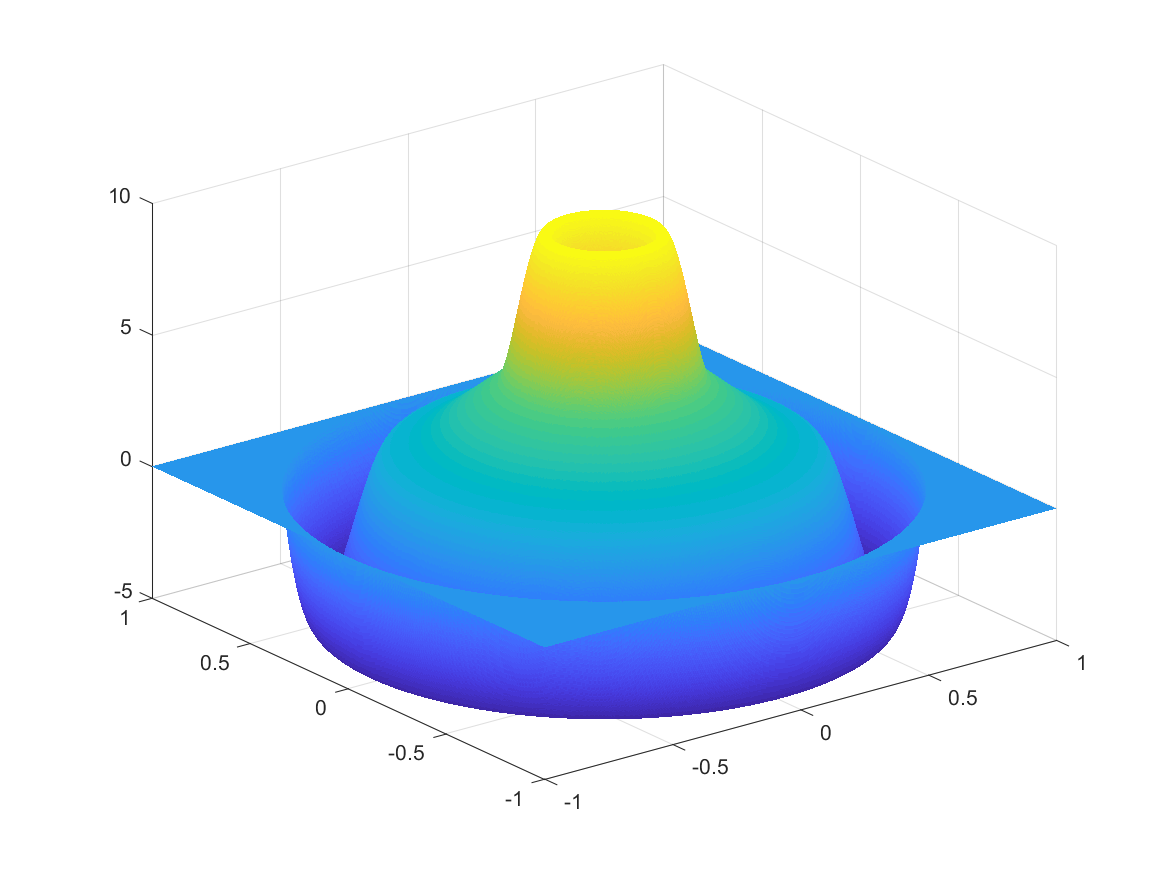
\includegraphics[trim = 40 30 30 30, clip, width=\linewidth]
      {pictures/chapExperiments/secExactSol/f04/inSi.png}
    \label{fig:f04InSi}
  \end{subfigure}
  \quad
  \begin{subfigure}[b]{.38\linewidth}
    \centering
    \caption{$f_\textrm{HR}$ entlang der x- und y-Achse}
    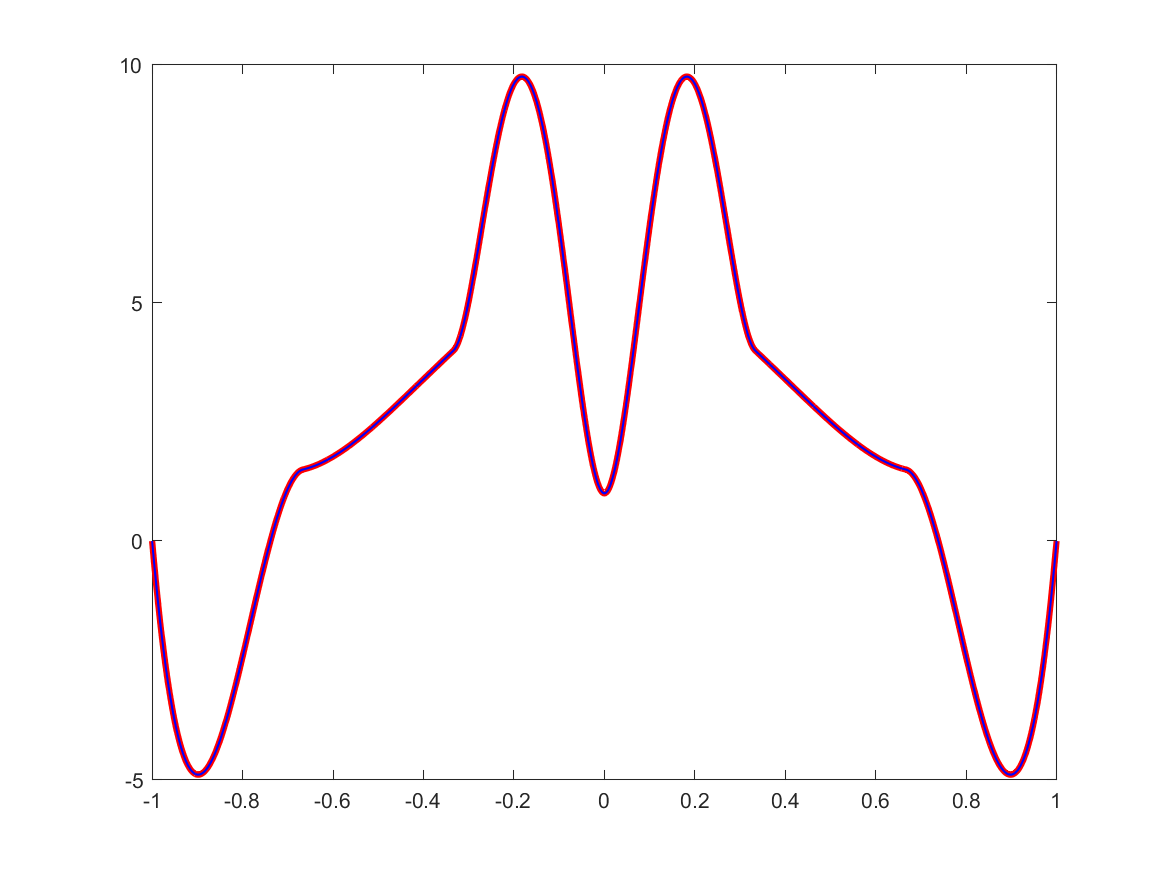
\includegraphics[trim = 50 30 50 20, clip, width=\linewidth]
      {pictures/chapExperiments/secExactSol/f04/inSiAxis.png}
    \label{fig:f04InSiAxis}
  \end{subfigure}

  \begin{subfigure}[b]{.38\linewidth}
    \centering
    \caption{$u_\textrm{HR}$}
    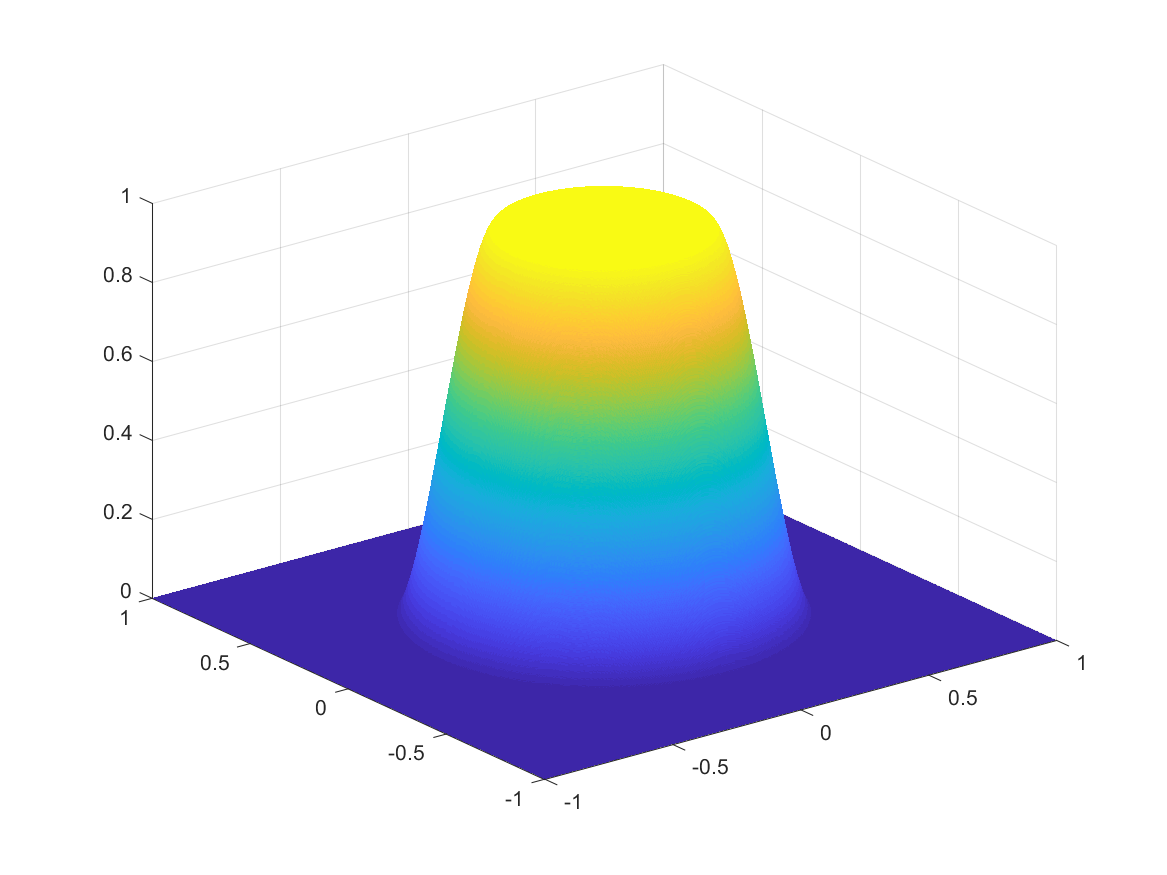
\includegraphics[trim = 40 30 30 30, clip, width=\linewidth]
      {pictures/chapExperiments/secExactSol/f04/exactSolution.png}
    \label{fig:f04ExactSol}
  \end{subfigure}
  \quad
  \begin{subfigure}[b]{.38\linewidth}
    \centering
    \caption{$u_\textrm{HR}$ entlang der x- und y-Achse}
    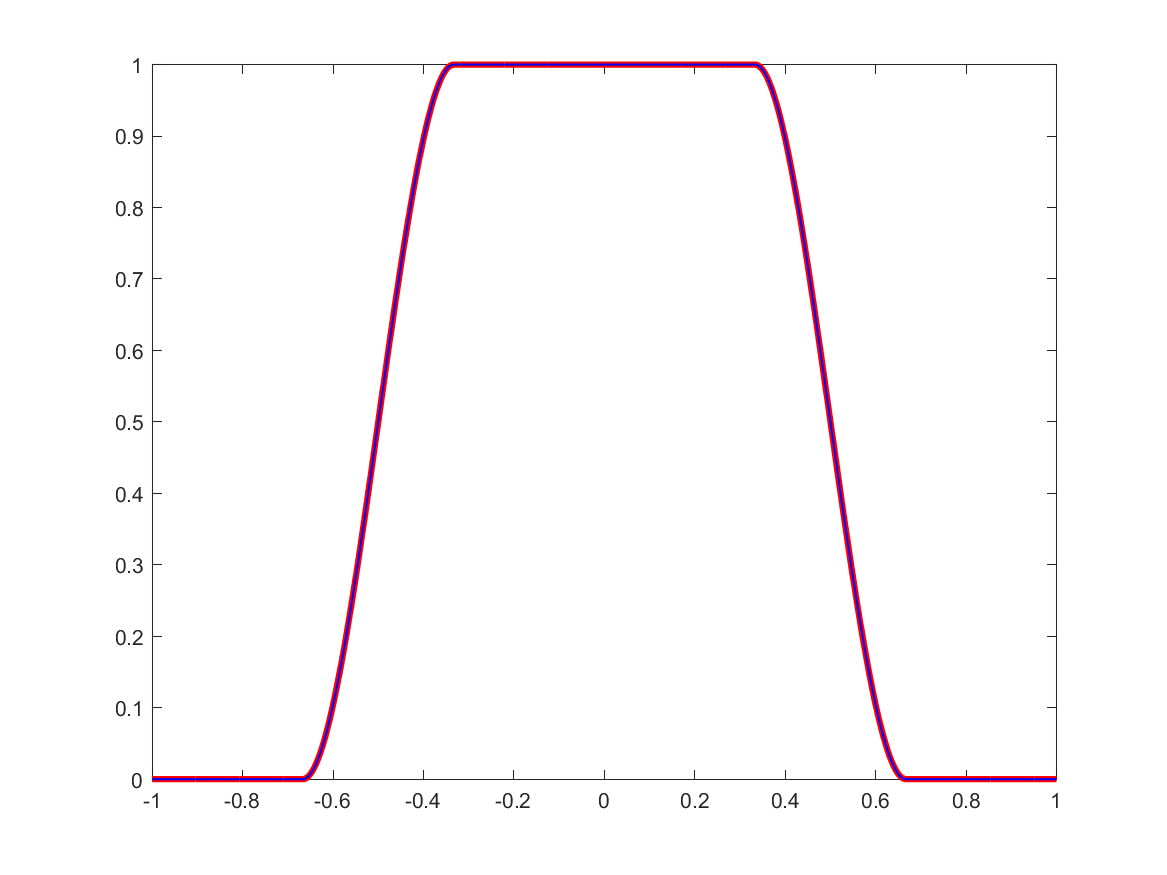
\includegraphics[trim = 50 30 50 20, clip, width=\linewidth]
      {pictures/chapExperiments/secExactSol/f04/exactSolutionAxis.png}
    \label{fig:f04ExactSolAxis}
  \end{subfigure} 
  \caption{Funktionen $f_\textrm{HR}$ und $u_\textup{HR}$ sowie deren
  Darstellungen entlang der x-Achse (blau) und der y-Achse (rot) für
  $\alpha = 1$}
  \label{fig:f04Plots}
\end{figure}
Dieses Eingangssignal und die exakte Lösung sind in \Cref{fig:f04Plots}
dargestellt.
\begin{figure}[p]
  \centering
  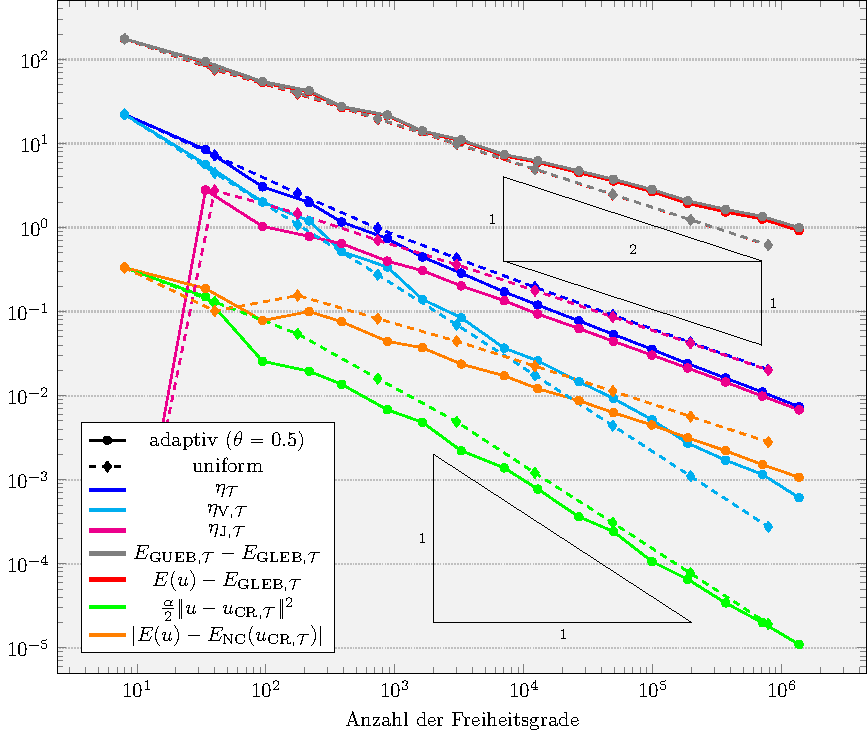
\includegraphics[width=.8\linewidth]
    {pictures/chapExperiments/secExactSol/f04/conv.pdf}
  \caption{Ergebnisse der Rechnungen mit adaptiver und uniformer 
    Netzverfeinerung für das Eingangssignal $f_\textup{HR}$}
  \label{fig:f04Convergence}
\end{figure}
Allerdings stellen wir in \Cref{fig:f04Convergence} lediglich fest, dass im
Vergleich zu \Cref{fig:f01Convergence} alle Graphen um einen Faktor von etwa
$10^{1/2}$ nach unten verschoben sind.
Insbesondere verändern sich die Konvergenzraten nicht.
Eine noch stärkere Regularitätsanname scheint die Raten also nicht weiter zu
verbessern, es werden aber geringfügig kleinere Werte erreicht.
Möglicherweise sind bei der hier benutzten Diskretisierung keine besseren Raten
erreichbar und die Betrachtung einer Methode höherer Ordnung wäre dazu
notwendig.

Nun betrachten wir noch einmal das Eingangssignal $f_1$, um den Einfluss der
Wahl von $\gamma\in(0,1]$ aus der \Cref{def:refinementIndicator} des
Verfeinerungsindikators $\etaT$ auf die Rechungen zu untersuchen.
Je kleiner die Wahl von $\gamma$, desto dominanter sollte nach Definition der
Einfluss von $\etaJ$ auf $\etaT$ sein und entsprechend dort stärker 
verfeinert werden, wo die Kantensprünge größer sind.
Dieser Effekt sollte auch für $\gamma=0$ zu beobachten sein, weshalb wir
diese Wahl ebenfalls untersuchen.
\begin{figure}[p]
  \centering
  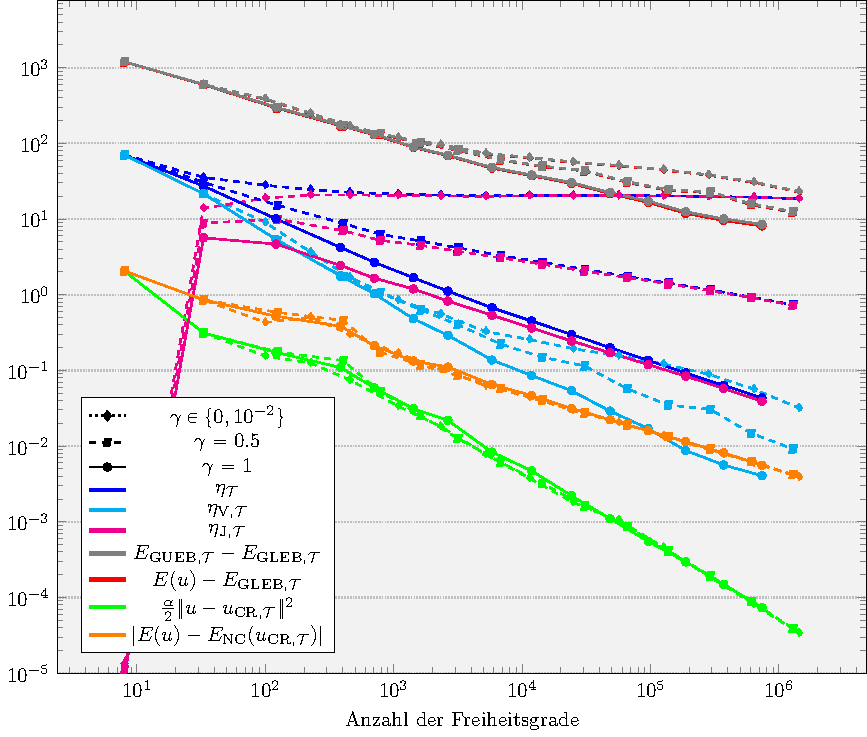
\includegraphics[width=.8\linewidth]
    {pictures/chapExperiments/secExactSol/parGamma/conv.pdf}
  \caption{Ergebnisse des Programms mit verschiedenen Werten von $\gamma$ für
    das Eingangssignal $f_1$, wobei die Graphen für $\gamma \in\{0,10^{-2}\}$
    nicht sichtbar unterscheidbar sind und deshalb nur der Graph für $\gamma=0$
    dargestellt ist}
  \label{fig:parGammaConvergence}
\end{figure}
In \Cref{fig:parGammaConvergence} ist tatsächlich zu erkennen, dass
$\etaJ$ mit kleinerem $\gamma$ deutlich größere Werte annimmt, sodass
sogar die Konvergenzrate von $\etaJ$ abnimmt. 
Da $\etaJ$ den Verfeinerungsindikator $\etaT$ dominiert, zeigt dieser das
gleiche Konvergenzverhalten.
Für $\gamma=0$ stagniert $\etaJ$ sogar.
Eine Erklärung für diese Beobachtungen ist, dass, wie bereits
festgestellt, die Sprungterme $\sum_{F\in\Ecal(\Tcal)}\Vert
[\ucrt]_F\Vert_{L^1(F)}$ nicht minimiert werden.
Insbesondere für $\gamma=0$ wird somit im Verfeinerungsindikator der Anteil
$\etaJ$ stark gewichtet, der in diesem Fall nicht gegen 0 konvergiert.  
Weiterhin ist die Konvergenzrate von $\etaV$ etwas schlechter, wenn $\gamma$
klein gewählt wird.
Die Fehlergraphen $\frac{\alpha}{2}\Vert u-\ucrt\Vert^2$ und
$|E(u)-\Enc(\ucrt)|$ zeigen allerdings für die verschiedenen Wahlen von
$\gamma$ keine nennenswerten Unterschiede. 
Die für den Verfeinerungsindikator suboptimalen Wahlen von $\gamma$ scheinen
also keinen negativen Effekt auf diese zu haben.
\begin{figure}[p]
  \centering
  \begin{subfigure}{.32\linewidth}
    \centering
    \caption{$\gamma=0$, $\text{nrDof}\approx 1\,440\,000 $}
    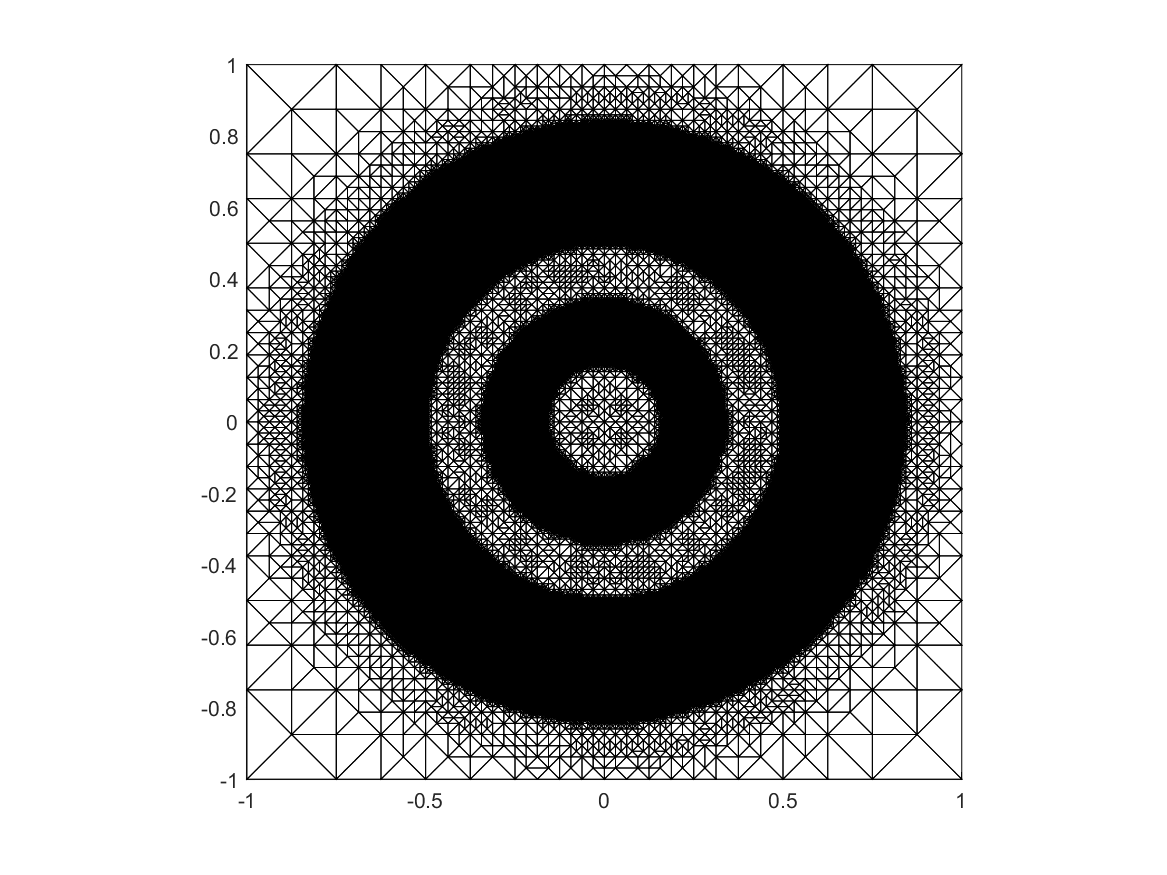
\includegraphics[trim = 100 30 80 20, clip, width=\linewidth]
      {pictures/chapExperiments/secExactSol/parGamma/0/lvl14/triangulation.png}
    \label{fig:gamma0Triang}
  \end{subfigure}
  \begin{subfigure}{.32\linewidth}
    \centering
    \caption{$\gamma=0.5$, $\text{nrDof}\approx 1\,280\,000$}
    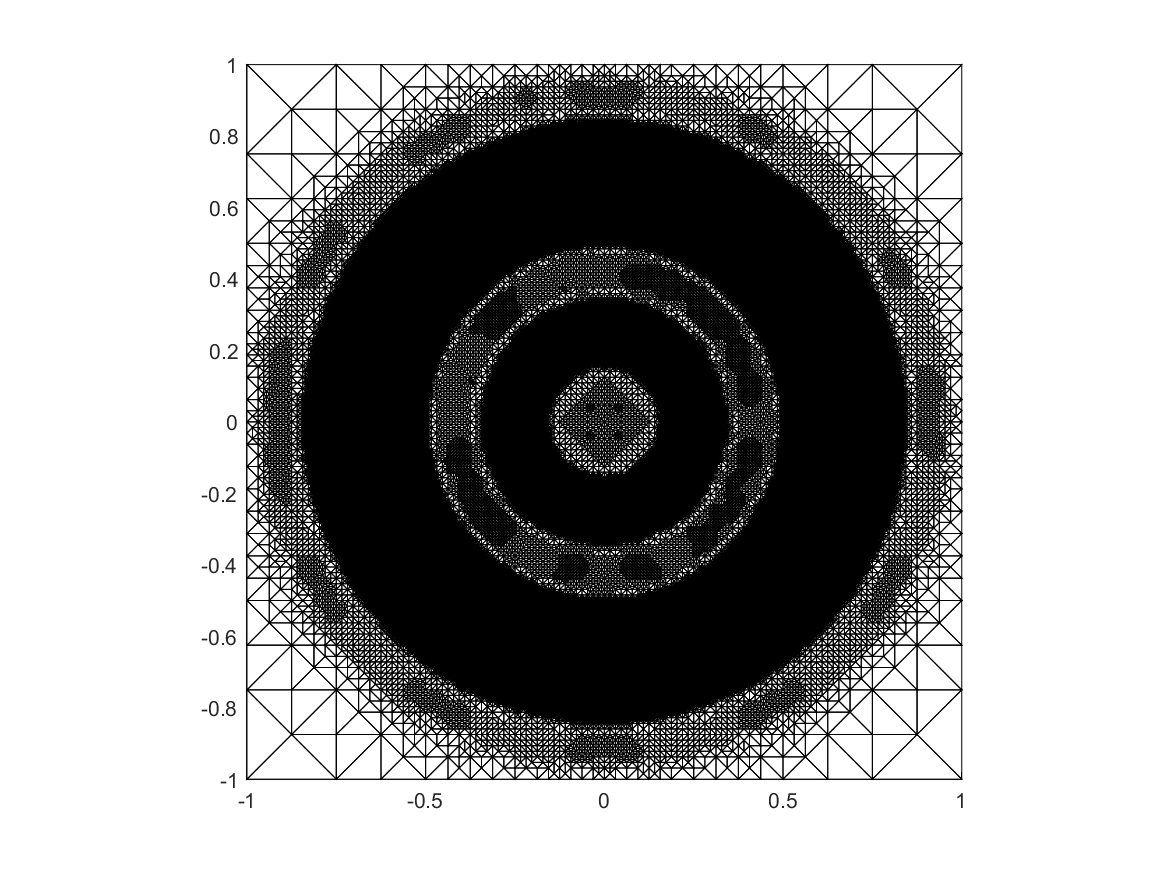
\includegraphics[trim = 100 30 80 20, clip, width=\linewidth]
      {pictures/chapExperiments/secExactSol/parGamma/5em1/lvl14/triangulation.png}
    \label{fig:gammaDot5Triang}
  \end{subfigure}
  \begin{subfigure}{.32\linewidth}
    \centering
    \caption{$\gamma=1$, $\text{nrDof}\approx 740\,000$}
    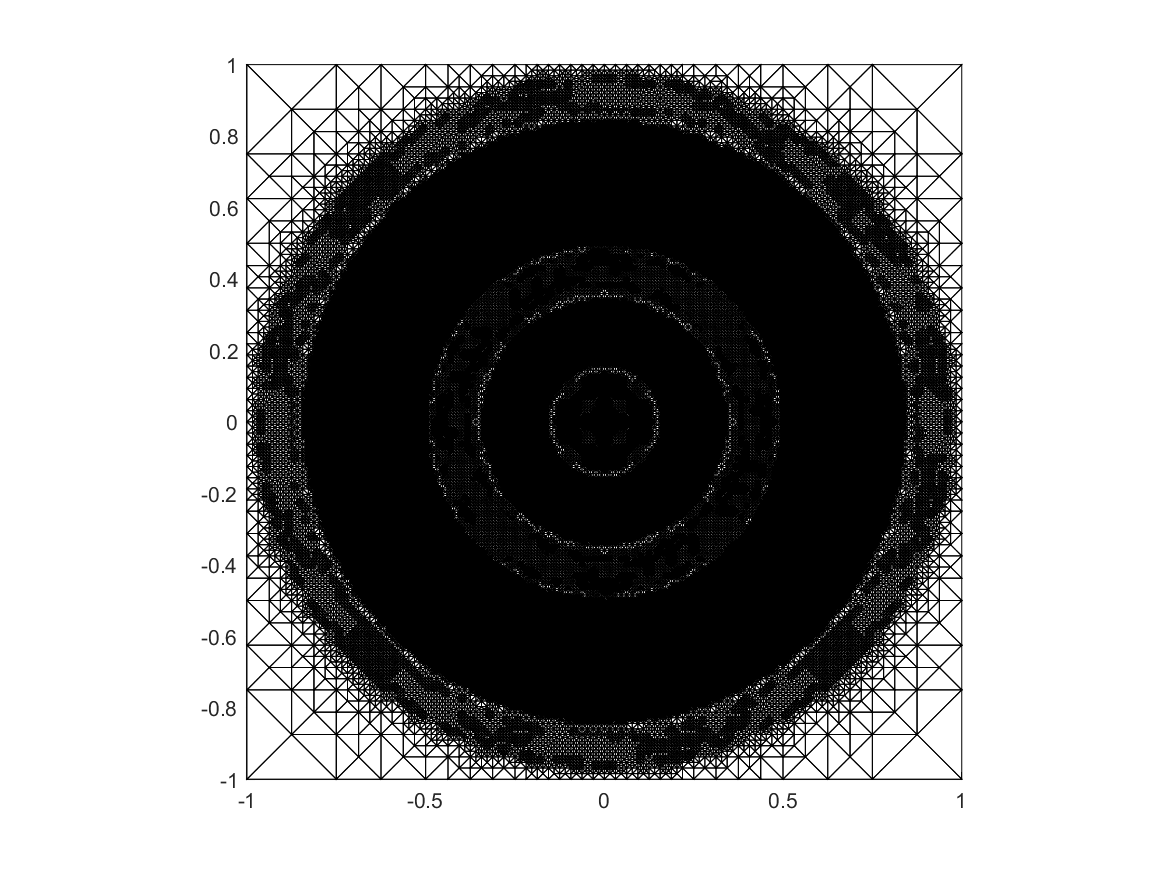
\includegraphics[trim = 100 30 80 20, clip, width=\linewidth]
      {pictures/chapExperiments/secExactSol/parGamma/1/lvl14/triangulation.png}
    \label{fig:gamma1Triang}
  \end{subfigure}
  \caption{Triangulierungen des jeweils letzten Levels 14 der Rechnungen mit
    verschiedenen Werten von $\gamma$ für das Eingangssignal $f_1$}
  \label{fig:gammaTriangs}
\end{figure}
In \Cref{fig:gammaTriangs} ist die Wirkung des Verfeinerungsindikators gut zu
erkennen. 
Die Kantensprünge sind dort am größten, wo die Lösung $u$, und damit die
meisten Iterate, nicht konstant sind.   
Dementsprechend wird mit kleinerem $\gamma$ stark dort verfeinert, wo die Lösung
$u$ aus \Cref{fig:f01Plots} nicht konstant ist.
Dies ist zu erkennen, obwohl die abgebildeten Triangulierungen für kleine
$\gamma$ deutlich mehr Freiheitsgrade haben als für $\gamma=1$.
Da wir im Experiment zu \Cref{fig:f01Convergence} bereits gesehen habe, dass
die Konvergenzraten bei adaptiver Netzverfeinerung nicht besser sind als bei
uniformer Netzverfeinerung, ist die ausbleibende Verbesserung der Ergebnisse
durch eine für $\gamma<1$ adaptivere Verfeinerung nicht unerwartet.
Insgesamt halten wir fest, dass die zu Beginn des Kapitels getroffene Wahl
von $\gamma=1$ weiterhin sinnvoll bleibt, da diese keinen Einfluss
auf die Fehlergraphen zu haben scheint, aber bessere Konvergenzraten
des Verfeinerungsindikators und seiner Anteile im Vergleich zu kleineren
Werten von $\gamma$ bewirkt.
Auch hier möchten wir anmerken, dass Ungleichung
\eqref{eq:expectedInequalities} für alle Wahlen von $\gamma$ erfüllt ist.

%\vspace{-.8mm}
Als nächstes wollen wir die Experimente mit Eingangssignal $f_1$ aus
\Cref{fig:f01Convergence} noch mit den Experimenten mit $\alpha=10^4$ und dem
Eingangssignal $f_{10^4}$ vergleichen.
\begin{figure}[p]
  \centering
  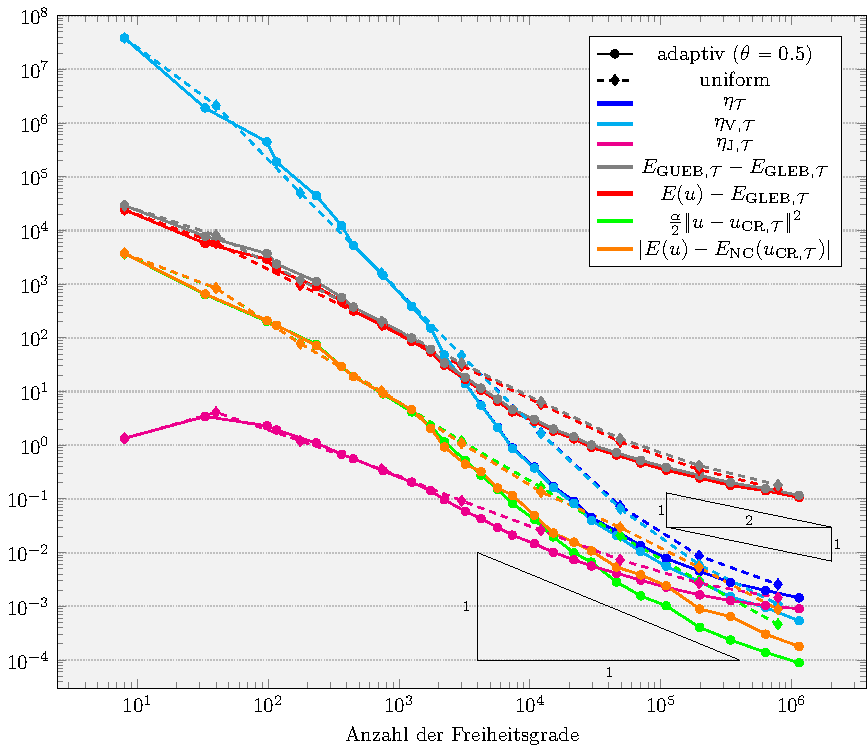
\includegraphics[width=.8\linewidth]
    {pictures/chapExperiments/secExactSol/f01LargeAlpha/conv.pdf}
  \caption{Ergebnisse der Rechnungen mit adaptiver und uniformer 
    Netzverfeinerung für das Eingangssignal $f_{10^4}$}
  \label{fig:f01LargeAlphaConvergence}
\end{figure}
Die Konvergenzraten für die Experimente mit Eingangssignal $f_{10^4}$ in
\Cref{fig:f01LargeAlphaConvergence} sind während eines vorasymptotischen
Bereichs, der bei etwa $10^5$ Freiheitsgraden endet, größer als bei
den Experimenten mit Eingangssignal $f_1$.
Danach sehen wir bei allen Graphen, außer dem für $|E(u)-\Enc(\ucrt)|$, die
anscheinend gleichen Raten, die wir schon in \Cref{fig:f01Convergence}
beobachtetet haben. 
Die Konvergenzrate von $|E(u)-\Enc(\ucrt)|$ scheint nun $1$ statt wie zuvor
1/2 zu sein.
Ansonsten gibt es nur zwei weitere nennenswerte Unterschiede.
Zum einen dominiert $\etaV$ hier lange den Verfeinerungsindikator, 
wobei ab etwa $10^6$ Freiheitsgraden die Dominanz von $\etaJ$ zu 
beginnen scheint, zum anderen erreichen alle Graphen, mit Ausnahme des
quadrierten exakten Fehlers und $\etaV$, geringere Werte nach $10^6$
Freiheitsgraden als für das Eingangssignal $f_1$.
Die Existenz des großen vorasymptotischen Bereichs wird möglicherweise dadurch
verursacht, dass für $\alpha=10^4$ alle Graphen, abgesehen von
$\etaJ$, zu Beginn des AFEM-Algorithmus deutlich größere Werte annehmen als für 
$\alpha =1$. 
Das Eingangssignal $f_{10^4}$ nimmt ebenfalls signifikant größere Werte an als
$f_1$.
Die Iterationen auf den ersten Leveln der AFEM-Routine erreichen dann jeweils
starke Reduktionen der betrachteten Terme und bedingen somit den
vorasymptotischen Bereich.
Die Ungleichung \eqref{eq:expectedInequalities} ist nach
\Cref{fig:f01LargeAlphaConvergence} auch hier stets gültig.

%\vspace{-.8mm}
Zum Abschluss dieses Abschnitts möchten wir für die betrachteten Experimente
mit den Eingangssignalen $f_1$, $f_{10^4}$ und $f_\textup{HR}$ die Anzahl der
Iterationen vergleichen.
\begin{figure}[p]
  \centering
  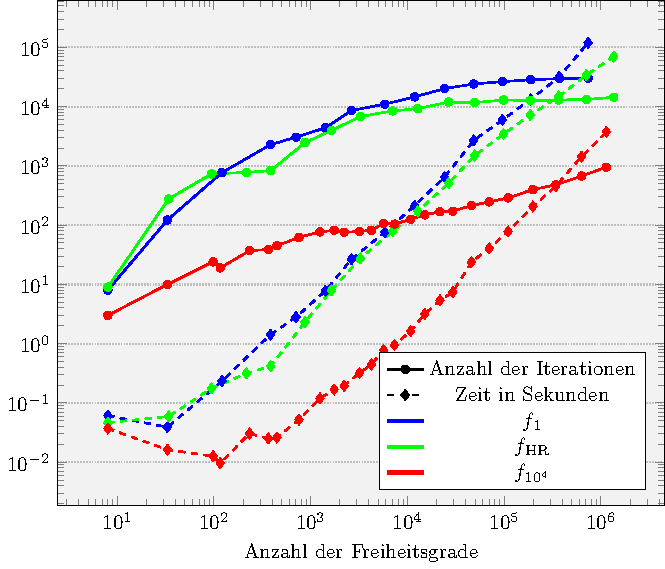
\includegraphics[width=.8\linewidth]
    {pictures/chapExperiments/secConclusion/nrIterComp/exactSol/misc.pdf}
  \caption{Anzahl der Iterationen und benötigte Zeit für die primalen-dualen
    Iterationen während des AFEM-Algorithmus bei den Rechnungen mit $\alpha=1$
    für die Eingangssignale $f_1$ und $f_\textup{HR}$ sowie bei der Rechnung mit
    $\alpha=10^4$ für das Eingangssignal $f_{10^4}$} 
  \label{fig:inSiNrIterComparison}
\end{figure}
In \Cref{fig:inSiNrIterComparison} ist zu erkennen, dass bis $10^6$
Freiheitsgrade das Beispiel mit Eingangssignal $f_{10^4}$, welches im Gegensatz
zu den anderen beiden Rechnungen den Parameter $\alpha=10^4$ nutzt, bei einer
vergleichbaren Anzahl von Freiheitsgraden deutlich weniger Iterationen
benötigt. 
Ähnlich zu \Cref{sec:choiceOfParameters} für den Parameter
$\tau$ könnte auch hier Ungleichung \eqref{eq:nrIterationsInequality}, deren
rechte Seite antiproportional zu $\alpha$ ist, der Grund für diese Beobachtung
sein.
%Auch dies stützt unsere Hypothese aus  zum
%Parmeter $\tau$, denn für den Parameter $\alpha$ lässt sich ebenfalls
%feststellen, dass sich die rechte Seite der Ungleichung
%\eqref{eq:nrIterationsInequality} antiproportional zu $\alpha$
%verhält, was weniger Iterationsschritte zur Folge haben sollte. 

\vfill


\section{Graufarbenbilder als Eingangssignale}
\label{sec:grayscalePicturesAsInputSignal}

In diesem Abschnitt wollen wir Ergebnisse von Experimenten untersuchen, bei
denen als Eingangssignal ein
Graufarbenbild nach \Cref{rem:grayscalePictureInputSignal} gegeben ist.
Für diese Rechnungen sind entsprechend weder exakte Lösung noch die schwache
Ableitung des Eingangssignals bekannt.
Zunächst betrachten wir das Eingangssignal \texttt{cameraman} aus
\Cref{fig:cameraman}. 
\begin{figure}[p]
  \centering
  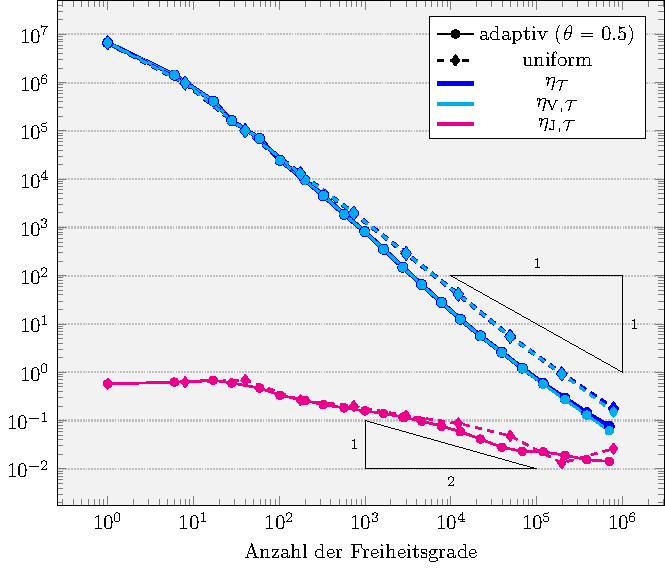
\includegraphics[width=.8\linewidth]
    {pictures/chapExperiments/secGrayscale/cam/conv.pdf}
  \caption{Ergebnisse der Rechnungen mit adaptiver und uniformer 
    Netzverfeinerung für das Eingangssignal \texttt{cameraman}}
  \label{fig:camConvergence}
\end{figure}
In \Cref{fig:camConvergence} sehen wir für den Verfeinerungsindikator $\etaT$
und dessen Anteil $\etaV$ die Konvergenzrate $1$.
Für den Anteil $\etaJ$ von $\etaT$ ist ungefähr die Rate $1/2$ zu erkennen, 
wobei $\etaJ$ bei uniformer Netzverfeinerung für das letzte Level einen
etwas größeren Wert annimmt als für das vorletzte.
Ansonsten ist bei den Konvergenzraten kein Unterschied zwischen uniformer und
adaptiver Netzverfeinerung festzustellen.
Die Raten von $\etaV$ und $\etaJ$ stimmen mit den Raten überein, die schon beim
Experiment mit Eingangssignal $f_1$ in \Cref{fig:f01Convergence} beobachtet
wurden, wobei hier der Verfeinerungsindikator von $\etaV$ dominiert wird und
nicht, wie beim Experiment mit Eingangssignal $f_1$, von $\etaJ$.
Dementsprechend konvergiert hier $\etaT$ auch nicht mit der Rate 1/2, sondern
mit der Rate $1$.
Weiterhin nimmt $\etaV$, und somit auch $\etaT$, im Vergleich zur Rechnung mit
Eingangssignal $f_1$ zu Beginn der AFEM-Routine deutlich höhere Werte an.
Diese sind vergleichbar mit den beim Experiment mit Eingangssignal $f_{10^4}$
in \Cref{fig:f01LargeAlphaConvergence}, bei dem ebenfalls $\alpha=10^4$ gewählt
war, beobachteten Werten. 
Bei einer Rechnung mit einem Eingangssignal $f$, bei dem $\alpha$ groß gewählt
ist im Vergleich zu einem anderen Experiment, scheinen also auf den ersten
Leveln der AFEM-Routine höhere Werte für $\etaV$ aufzutreten als in einem
Experiment mit einer kleineren Wahl von $\alpha$.
\begin{figure}[p]
  \centering
  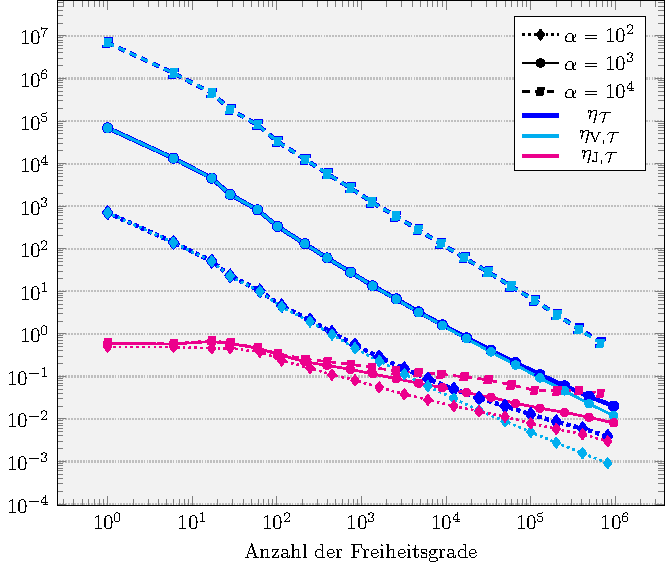
\includegraphics[width=.8\linewidth]
    {pictures/chapExperiments/secGrayscale/denoise/conv.pdf}
  \caption{Ergebnisse der Rechnungen zu \Cref{fig:exampleDenoising} für drei
    verschiedene Werte von $\alpha$}
  \label{fig:denoiseConvergence}
\end{figure}
Dies wird bekräftigt in \Cref{fig:denoiseConvergence}, in der wir die
Konvergenzgraphen zu den Experimenten aus \Cref{fig:exampleDenoising}
vergleichen für $\alpha\in\{10^2,10^3,10^4\}$ und ebendieses Verhalten
beobachten.
Ein Grund dafür könnte sein, dass, wenn $\alpha$ groß gewählt wird, die Terme
$\Vert f-\alpha \ucrt\Vert^2_{L^2(T)}$ im Anteil $\etaV$ des
Verfeinerungsindikators aus \Cref{def:refinementIndicator} für viele Dreiecke
$T\in\Tcal$ ebenfalls größere Werte annehmen als für ein Experiment mit einer
kleineren Wahl für $\alpha$.
\begin{figure}[p]
  \centering
  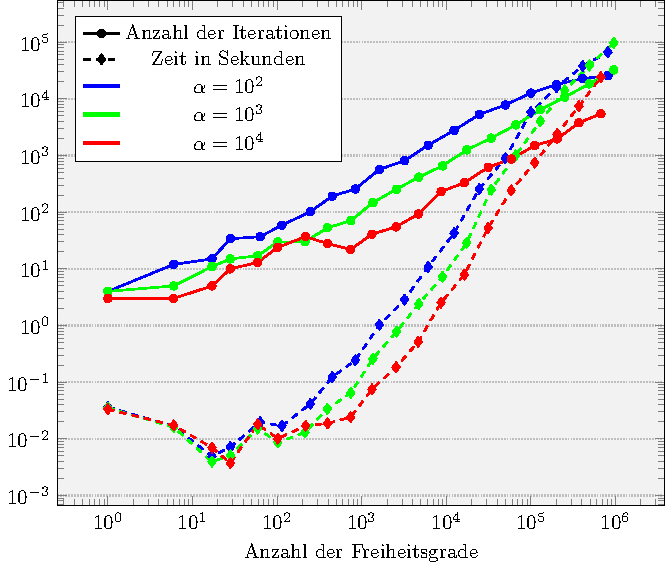
\includegraphics[width=.5\linewidth]
    {pictures/chapExperiments/secConclusion/nrIterComp/grayscale/misc.pdf}
  \caption{Anzahl der Iterationen und benötigte Zeit für die primalen-dualen
    Iterationen während des AFEM-Algorithmus bei den Rechnungen zu
    \Cref{fig:exampleDenoising} für drei verschiedene Werte von $\alpha$}  
  \label{fig:denoiseNrIterComparison}
\end{figure}
Weiterhin können wir durch die benötigte Anzahl der Iterationen für jedes Level
der Experimente zu \Cref{fig:exampleDenoising} in
\Cref{fig:denoiseNrIterComparison} noch einmal unsere Hypothese aus 
\Cref{sec:choiceOfParameters} zur Ungleichung \eqref{eq:nrIterationsInequality}
stützen, denn auch in \Cref{fig:denoiseNrIterComparison} benötigt die
primale-duale Iteration für eine größere Wahl von $\alpha$ weniger
Iterationsschritte.

Zum Abschluss diese Abschnitts möchten wir anhand des Beispiels mit
Eingangssignal \texttt{cameraman} die Wirkung des Verfeinerungsindikators
veranschaulichen.
\begin{figure}[p]
  \centering
  \begin{subfigure}[b]{.39\linewidth}
    \centering
    \caption{Triangulierung Level 17}
    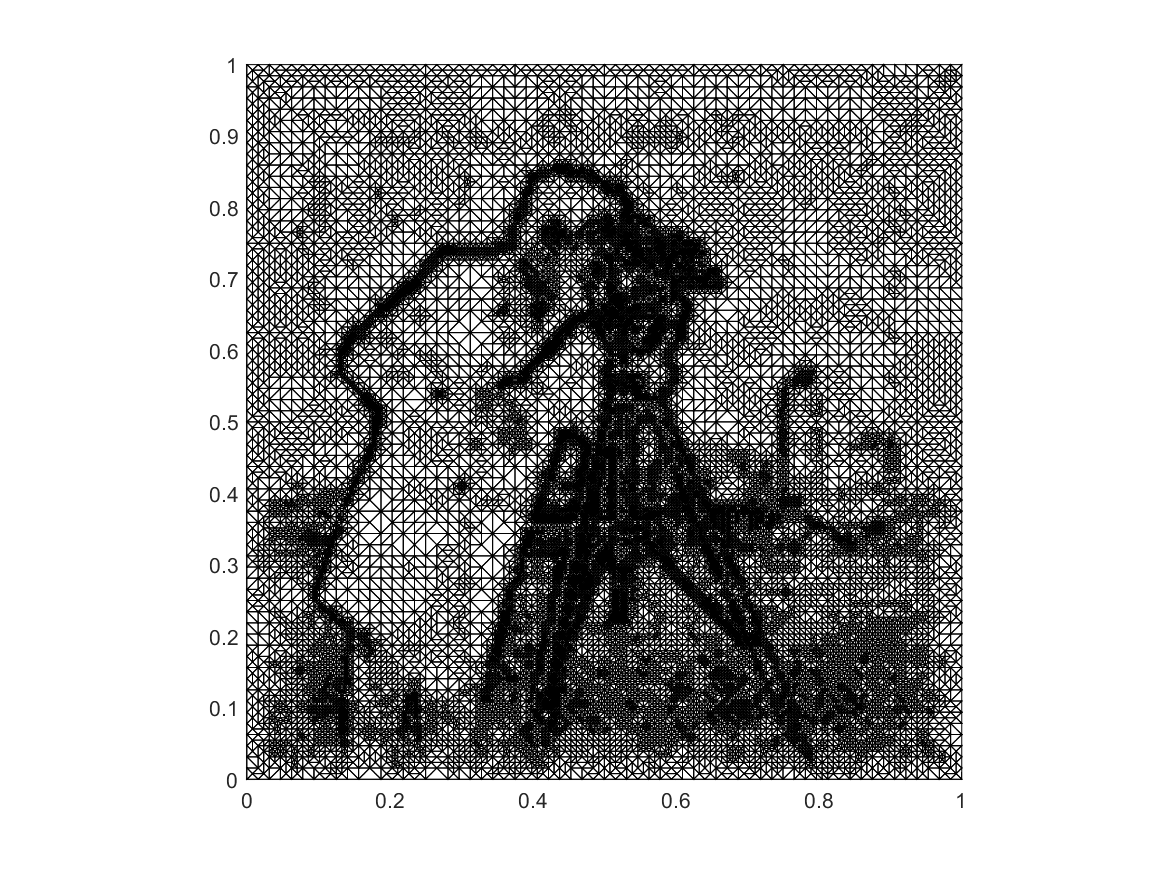
\includegraphics[trim = 100 30 80 20, clip, width=\linewidth]
      {pictures/chapExperiments/secGrayscale/cam/adaptive/lvl17/triangulation.png}
    \label{fig:camLvl17Triang}
  \end{subfigure}
  \quad
  \begin{subfigure}[b]{.39\linewidth}
    \centering
    \caption{Lösung Level 17}
    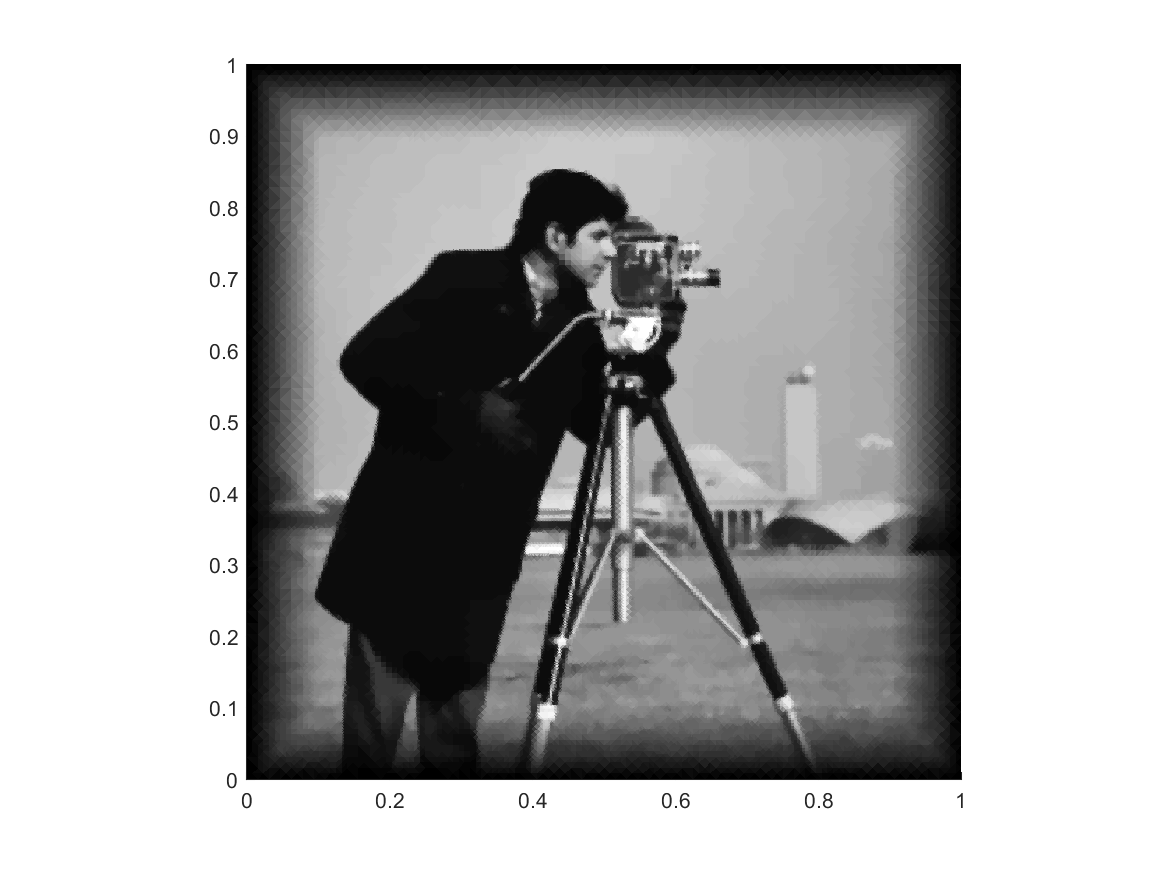
\includegraphics[trim = 100 30 80 20, clip, width=\linewidth]
      {pictures/chapExperiments/secGrayscale/cam/adaptive/lvl17/solutionGrayscale.png}
    \label{fig:camLvl17Sol}
  \end{subfigure}

  \begin{subfigure}[b]{.39\linewidth}
    \centering
    \caption{Triangulierung Level 21}
    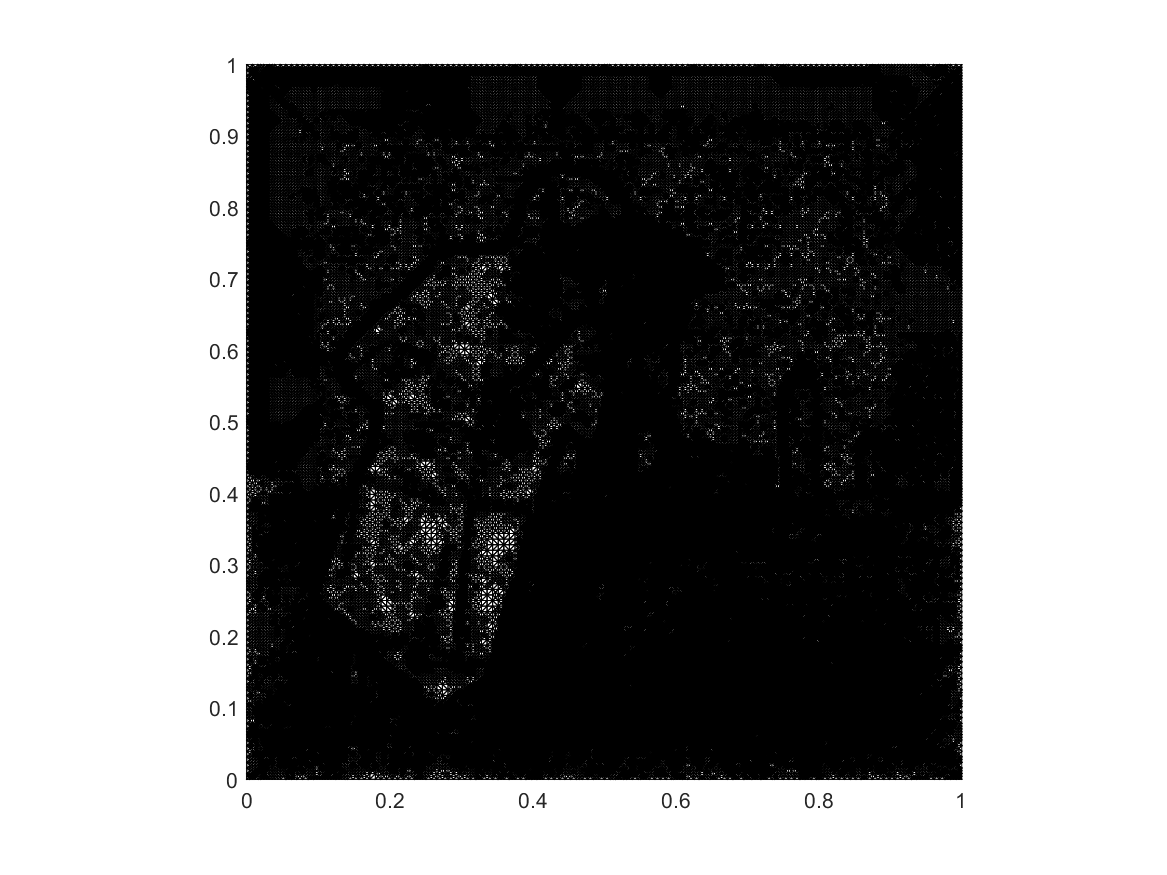
\includegraphics[trim = 100 30 80 20, clip, width=\linewidth]
      {pictures/chapExperiments/secGrayscale/cam/adaptive/lvl21/triangulation.png}
    \label{fig:camLvl21Triang}
  \end{subfigure}
  \quad
  \begin{subfigure}[b]{.39\linewidth}
    \centering
    \caption{Lösung Level 21}
    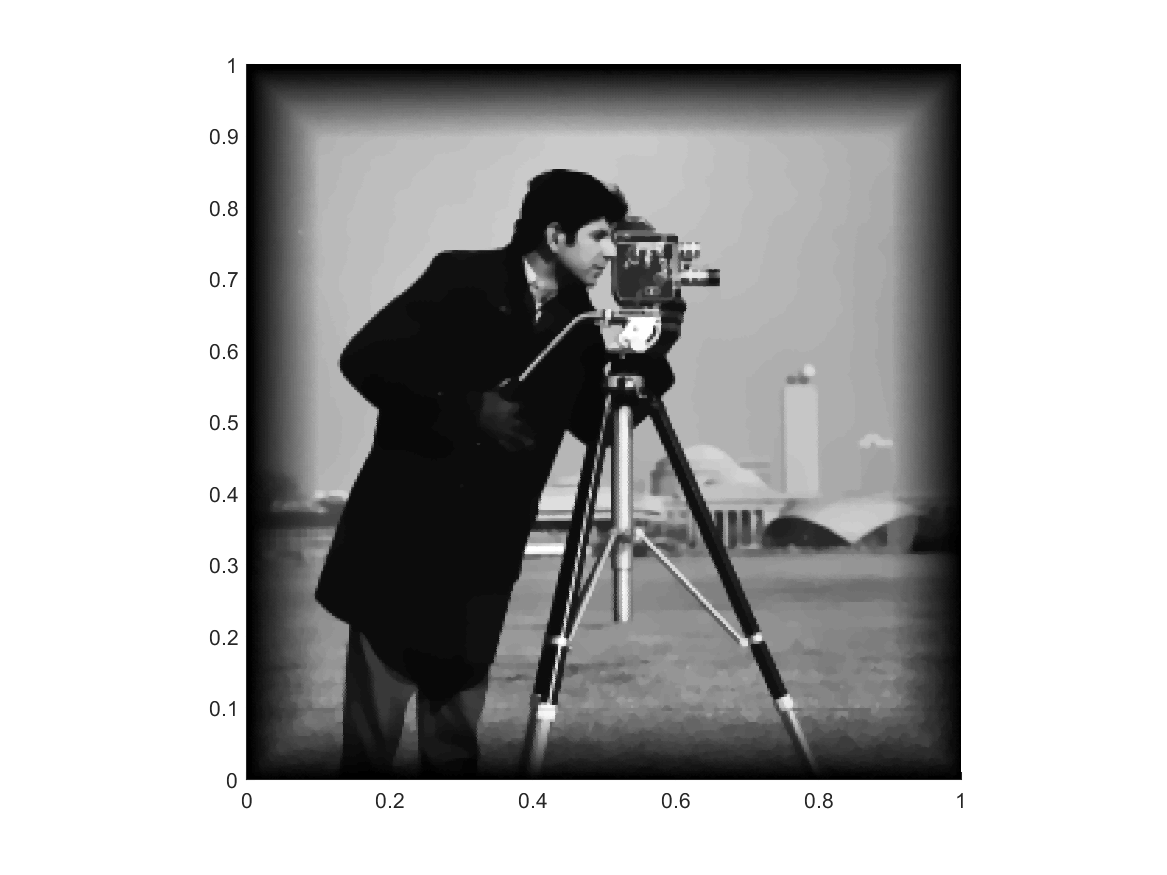
\includegraphics[trim = 100 30 80 20, clip, width=\linewidth]
      {pictures/chapExperiments/secGrayscale/cam/adaptive/lvl21/solutionGrayscale.png}
    \label{fig:camLvl21Sol}
  \end{subfigure}
  \caption{Triangulierung und diskrete Lösung, als Graufarbenplot aus der
    Draufsicht, nach der Rechnung mit Eingangssignal \texttt{cameraman} für
    Level 17 des AFEM-Algorithmus nach etwa 70\,000 Freiheitsgraden und für
    Level 21 nach etwa 700\,000 Freiheitsgraden}
  \label{fig:camTriang}
\end{figure}
Wir sehen in \Cref{fig:camLvl17Triang} gut, dass dieser eine Verfeinerung zu
den Unstetigkeiten bewirkt, insbesondere zu denen entlang deutlicher
Farbkontraste.
Außerdem ist zu erkennen, dass der hinzufügte graduelle Übergang zu schwarzem
Rand für das Eingangssignal den gewünschten Effekt hat, eine starke
Verfeinerung zum Rand, die aufgrund der angenommenen Nullranddaten passieren
würde, zu verhindern.
Somit wird tatsächlich dort stark verfeinert, wo mehr Informationen benötigt
werden, was am Rand nicht der Fall wäre.
Auch in \Cref{fig:camLvl21Triang} kann man, trotz der hohen Anzahl an
Freiheitsgaden, noch erkennen, wo es im Bild kaum Farbkontraste gibt und eine
Verfeinerung deshalb nicht unbedingt nötig ist.
Die diskrete Lösung ähnelt dem Eingangssignal, was aufgrund der großen Wahl für
$\alpha$ nach der Interpretation des ROF-Modellproblems aus
\Cref{chap:introduction} zu erwarten war.


\section{Stetige Approximation eines unstetigen Eingangssignals}

Im vorherigen \Cref{sec:grayscalePicturesAsInputSignal} konnten wir mangels
bekannter exakter Lösungen und schwacher Gradienten der Eingangssignale für die
Experimente nur die Konvergenzraten des Verfeinerungsindikators und seiner
Anteile $\etaV$ und $\etaJ$ untersuchen.
Da wir für $\etaV$ und $\etaJ$ die gleichen Raten wie für die Experimente in
\Cref{sec:experimentsWithExactSolution} beobachten konnten, interessiert uns,
ob andere Konvergenzraten ebenfalls vergleichbar sind zwischen Experimenten mit
stetigen Eingangssignalen und solchen mit unstetigen Eingangssignalen.
Deshalb möchten wir nun ein weiteres Beispiel mit einem unstetigen
Eingangssignal, welches wir durch eine nach \Cref{sec:constructionInputSignal}
konstruierte stetige Funktion approximieren können, betrachten.
Für die Rechnungen mit dieser stetigen Approximation als Eingangssignal kennen
wir die exakte Lösung sowie die schwachen Gradienten und können durch
die Konvergenzraten der entsprechenden Graphen möglicherweise Rückschlüsse
für die Raten der Rechnungen mit unstetigen Eingangssignalen ziehen.
Wir nutzen für alle Experimente in diesem Abschnitt als initiale Triangulierung
\texttt{BigSquare} aus \Cref{fig:triangBigSquare}.
Als unstetiges Eingangssignal, das als Graufarbenbild interpretiert einem 
weißen Kreis mit Radius $\frac{1}{2}$ entspricht, betrachten wir die Funktion
\begin{align*}
  f_\textrm{DC}(r)\coloneqq 
  \begin{cases}
    10^4, 
    & \text{falls } r\in \left[0,\frac{1}{2}\right]\!,\\
    0, 
    & \text{falls } r\in \left(\frac{1}{2},\infty\right)\!.
  \end{cases}
\end{align*}
Betrachten wir nun für einen Parameter $\beta\in(0,1)$ die Funktion
\begin{align*}
  u_\textrm{C}(r)\coloneqq 
  \begin{cases}
    1, 
    & \text{falls } r\in \left[0,\frac{1-\beta}{2}\right]\!,\\
    -\frac{1}{\beta}r + \frac{1+\beta}{2\beta}, 
    & \text{falls } r\in \left(\frac{1-\beta}{2}, \frac{1+\beta}{2}\right]\!,\\
    0,
    & \text{falls } r\in \left(\frac{1+\beta}{2},\infty\right)\!,
  \end{cases}
\end{align*}
so ist diese mit der Wahl
\begin{align*}
  \sgn(\partial_r u_\textrm{C}(r)) 
  &\coloneqq 
  \begin{cases}
    \frac{4}{1-\beta}r\left(\frac{1}{1-\beta}r -1\right)\!, 
    & \text{falls } r\in \left[0,\frac{1-\beta}{2}\right]\!,\\
    -1,
    & \text{falls } r\in \left(\frac{1-\beta}{2}, \frac{1+\beta}{2}\right]\!,\\
    \frac{4}{(\beta-1)^3}
    \left( 4r^3-3(\beta+3)r^2 +6(\beta+1)r-3\beta-1\right)\!, 
    & \text{falls } r\in \left(\frac{1+\beta}{2},\infty\right)\!,
  \end{cases}
\end{align*}
Lösung von \Cref{prob:continuousProblem} mit Eingangssignal
\begin{align*}
  f_\textrm{C}(r)\coloneqq 
  \begin{cases}
    \alpha - \frac{4}{1-\beta}\left(\frac{3}{1-\beta}r - 2\right)\!, 
    & \text{falls } r\in \left[0,\frac{1-\beta}{2}\right]\!,\\
    -\frac{\alpha}{\beta}\left( r-\frac{1+\beta}{2} \right) +\frac{1}{r}, 
    & \text{falls } r\in \left(\frac{1-\beta}{2}, \frac{1+\beta}{2}\right]\!,\\
    \frac{-4}{(\beta-1)^3}
    \left( 16r^2 -9(\beta+3)r + 12(\beta+1) - \frac{3\beta+1}{r}\right)\!, 
    & \text{falls } r\in \left(\frac{1+\beta}{2},\infty\right)\!.
  \end{cases}
\end{align*}
Die schwachen Gradienten von $u_\textup{C}$ und $f_\textup{C}$ können durch die
partiellen Ableitungen 
\begin{align*}
  \partial_r f_\textrm{C}(r) &= 
  \begin{cases}
    -\frac{12}{(1-\beta)^2},
    & \text{falls } r\in \left[0,\frac{1-\beta}{2}\right]\!,\\
    -\frac{\alpha}{\beta}-\frac{1}{r^2},
    & \text{falls } r\in \left(\frac{1-\beta}{2}, \frac{1+\beta}{2}\right]\!,\\
    -\frac{4}{(1-\beta)^3}\left( 32r-9(\beta+3)+\frac{3\beta+1}{r^2} \right)\!,
    & \text{falls } r\in \left(\frac{1+\beta}{2},\infty\right)\!,
  \end{cases}
\end{align*}
und
\begin{align*}
  \partial_r u_\textrm{C}(r) &= 
  \begin{cases}
    0,
    & \text{falls } r\in \left[0,\frac{1-\beta}{2}\right]\!,\\
    -\frac{1}{\beta},
    & \text{falls } r\in \left(\frac{1-\beta}{2}, \frac{1+\beta}{2}\right]\!,\\
    0,
    & \text{falls } r\in \left(\frac{1+\beta}{2},\infty\right)\!,
  \end{cases}
\end{align*}
bestimmt werden.
Wir wählen für unsere Experimente $\alpha = 10^4$ und $\beta = 10^{-3}$ und 
erhalten damit als Energie der exakten Lösung $E(u)\approx -3\,924.37413$.
\begin{figure}[p]
  \centering
  \begin{subfigure}[b]{.48\linewidth}
    \centering
    \caption{$f_\textup{C}$ entlang der Achsen}
    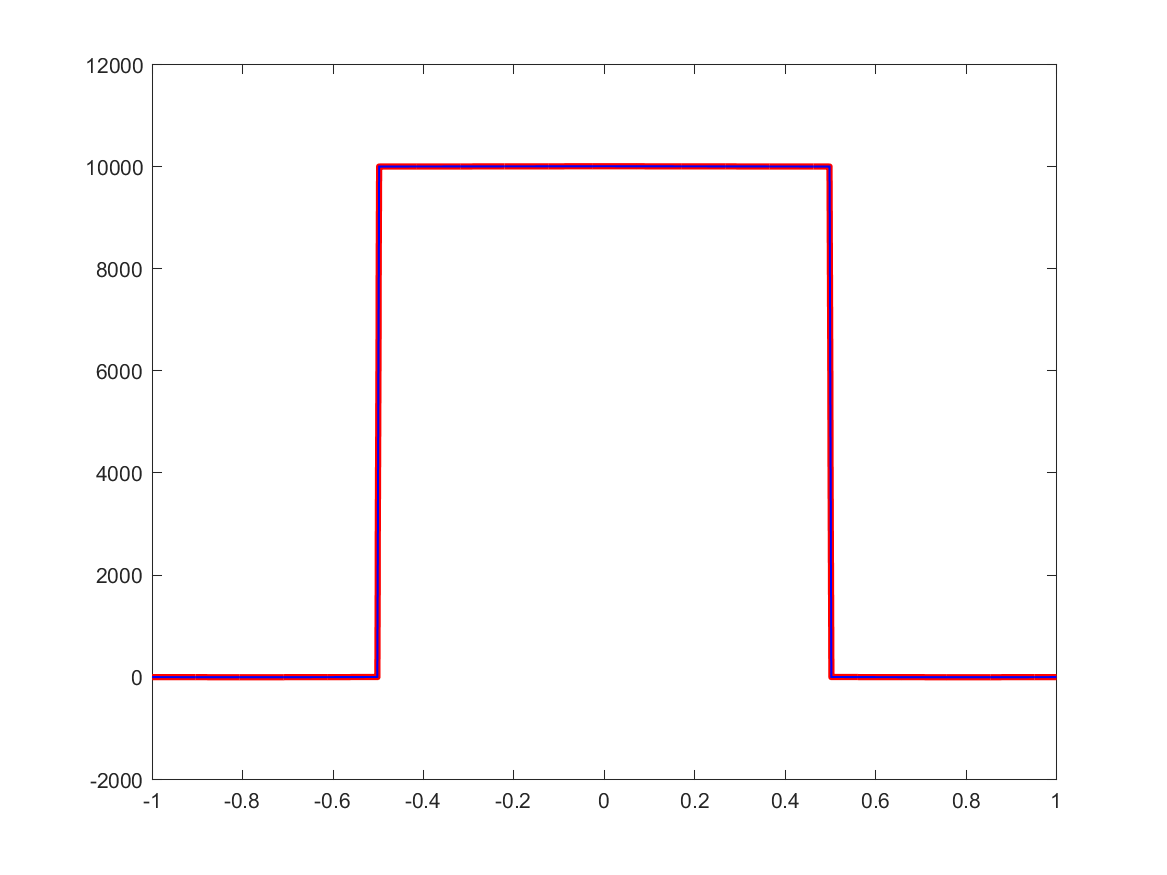
\includegraphics[trim = 40 30 50 20, clip, width=\linewidth]
      {pictures/chapExperiments/secGrayscale/circ/cont/inSiAxis.png}
    \label{fig:circContInSiAxis}
  \end{subfigure}
  \quad
  \begin{subfigure}[b]{.48\linewidth}
    \centering
    \caption{$u_\textup{C}$ entlang der Achsen}
    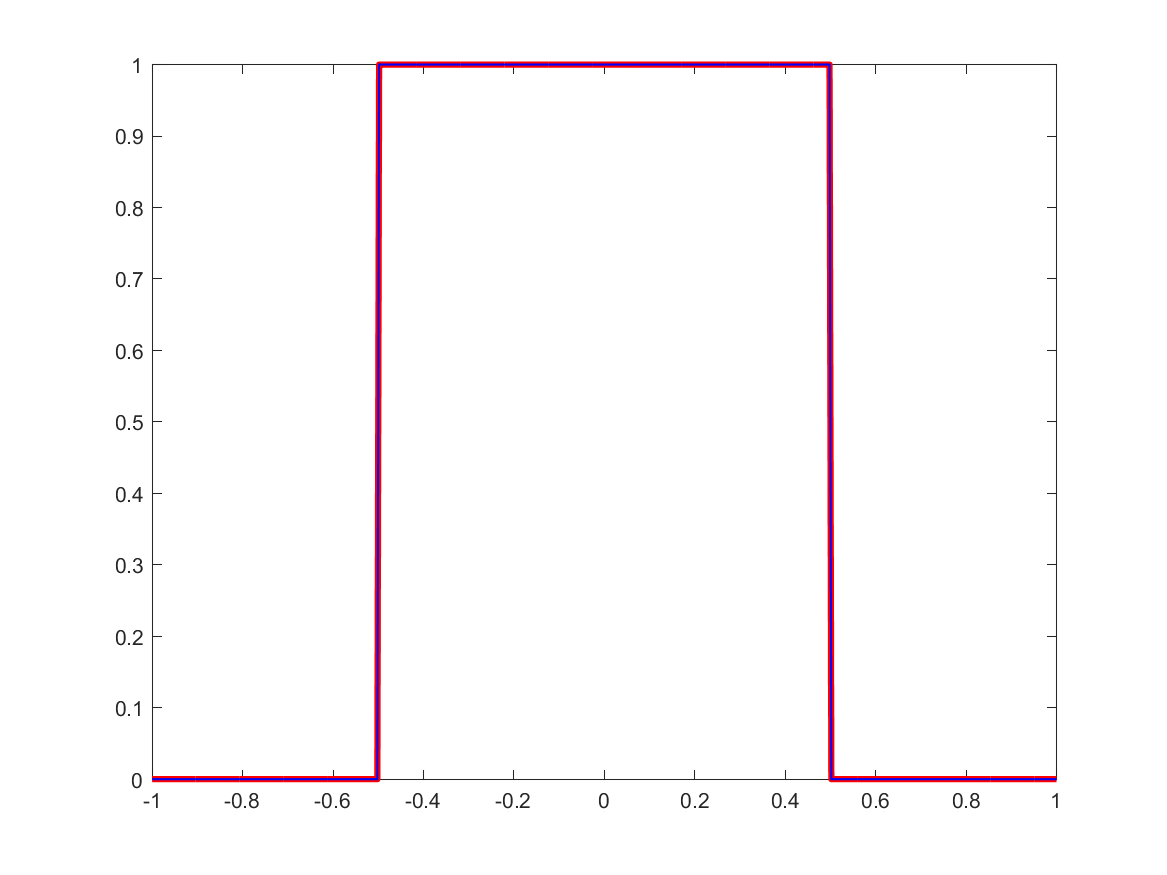
\includegraphics[trim = 40 30 50 20, clip, width=\linewidth]
      {pictures/chapExperiments/secGrayscale/circ/cont/exactSolutionAxis.png}
    \label{fig:circContExactSolAxis}
  \end{subfigure}
  \caption{Funktionen $f_\textup{C}$ und $u_\textup{C}$ entlang der x-Achse
    (blau) und der y-Achse (rot) für $\alpha = 10^4$ und $\beta = 10^{-3}$}
  \label{fig:circContPlotsAxis}
\end{figure}
Augenscheinlich ist $f_\textrm{C}$ für diese Wahl von $\alpha$ und $\beta$
tatsächlich eine stetige Approximation von $f_\textrm{DC}$, wie in
\Cref{fig:circContInSiAxis} zu sehen ist.
Außerdem sehen wir in \Cref{fig:circContPlotsAxis} für diese große Wahl von
$\alpha$ noch einmal, dass das Eingangssignal $f_\textup{C}$ ungefähr gleich
dem Produkt aus $\alpha$ und der exakten Lösung $u_\textup{C}$ zu sein scheint,
wie wir nach \Cref{chap:introduction} erwartet haben.
\begin{figure}[p]
  \centering
  \begin{subfigure}[b]{.48\linewidth}
    \centering
    \caption{adaptiv}
    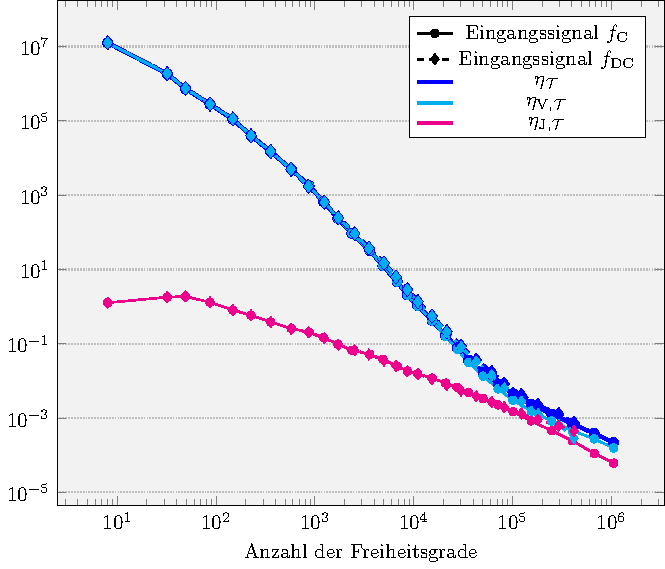
\includegraphics[width=\linewidth]
      {pictures/chapExperiments/secGrayscale/circ/convAdap.pdf}
    \label{fig:circConvAdaptive}
  \end{subfigure}
  \quad
  \begin{subfigure}[b]{.48\linewidth}
    \centering
    \caption{uniform}
    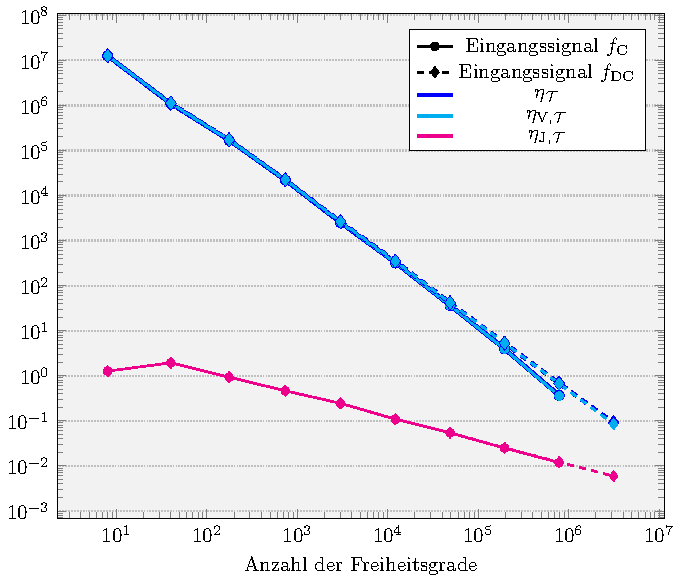
\includegraphics[width=\linewidth]
      {pictures/chapExperiments/secGrayscale/circ/convUnif.pdf}
    \label{fig:circConvUniform}
  \end{subfigure}
  \caption{Vergleich des Verfeinerungsindikators und seiner Anteile zwischen
    den Rechnungen mit Eingangssignal $f_\textup{C}$ und $f_\textup{DC}$ bei
    adaptiver (a) und uniformer (b) Netzverfeinerung}
  \label{fig:circConvComparison}
\end{figure}
Zunächst bestätigt \Cref{fig:circConvComparison} sowohl für adaptive
als auch uniforme Netzverfeierung, dass es zwischen den Experimenten mit
den Eingangssignalen $f_\textup{C}$ und $f_\textup{DC}$ bis etwa $10^6$
Freiheitsgrade keine deutlichen Unterschiede in der Entwicklung des
Verfeinerungsindikators und seiner Anteile gibt. 
\begin{figure}[p]
  \centering
  \begin{subfigure}[b]{.38\linewidth}
    \centering
    \caption{Eingangssignal $f_\textup{C}$}
    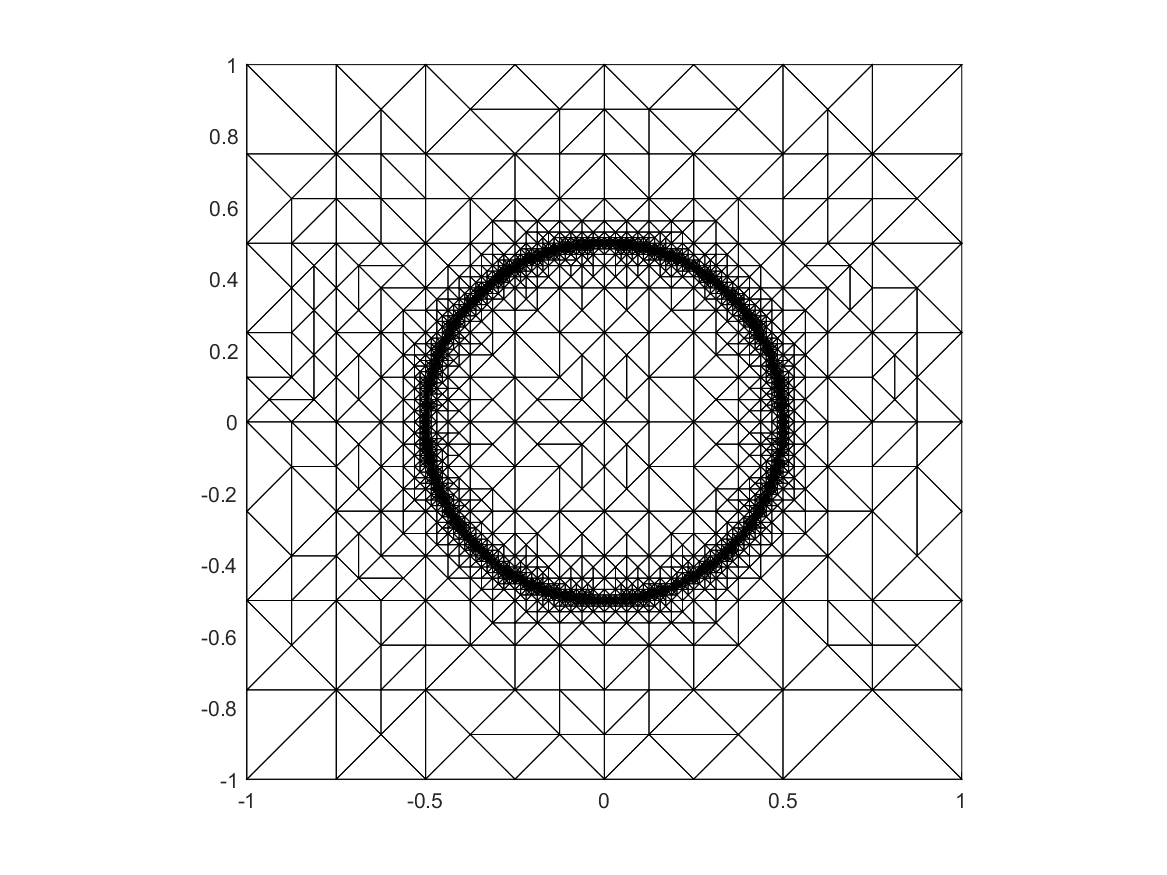
\includegraphics[trim = 100 30 80 20, clip, width=\linewidth]
      {pictures/chapExperiments/secGrayscale/circ/cont/adaptive/lvl17/triangulation.png}
    \label{fig:circContLvl17Triang}
  \end{subfigure}
  \quad
  \begin{subfigure}[b]{.38\linewidth}
    \centering
    \caption{Eingangssignal $f_\textup{DC}$}
    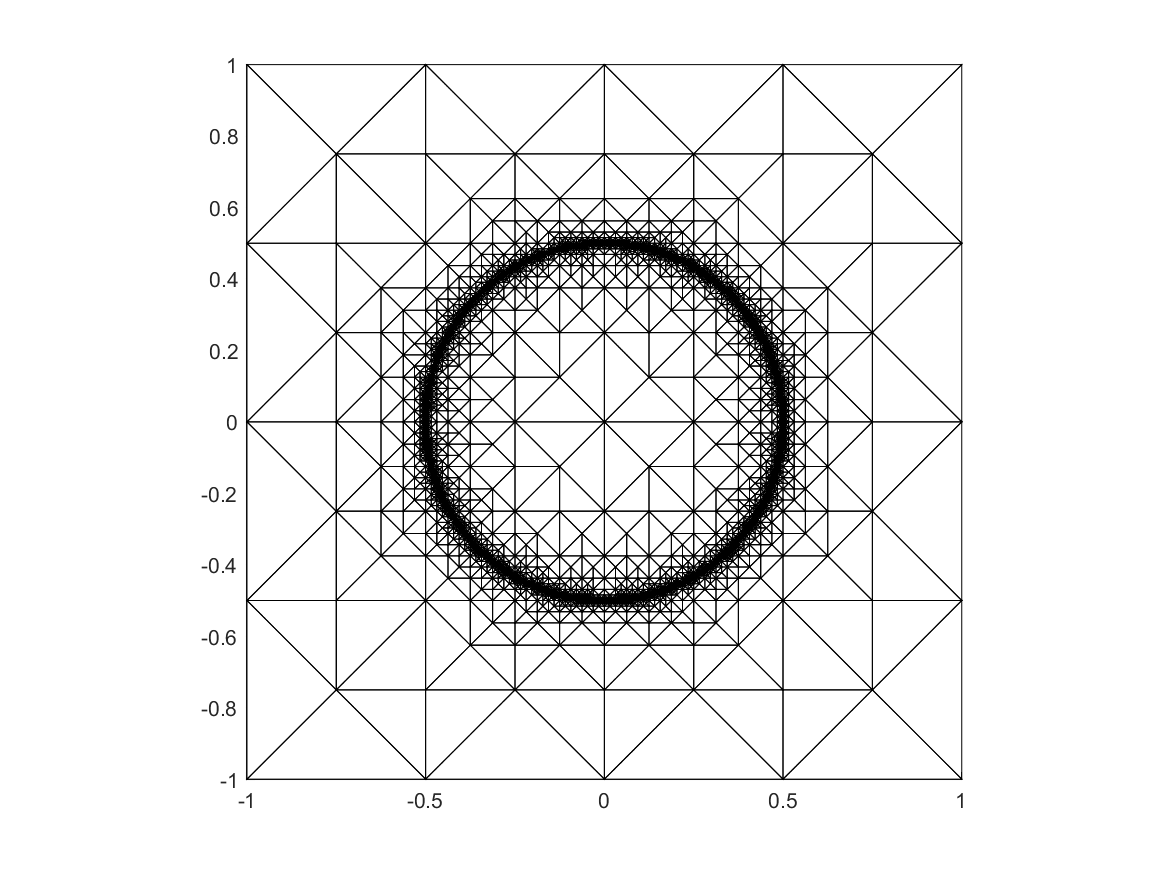
\includegraphics[trim = 100 30 80 20, clip, width=\linewidth]
      {pictures/chapExperiments/secGrayscale/circ/disc/adaptive/lvl17/triangulation.png}
    \label{fig:circDiscLvl17Triang}
  \end{subfigure}
  \caption{Triangulierungen nach den Rechnungen mit Eingangssignal
    $f_\textup{C}$ und $f_\textup{DC}$ für Level 17 des jeweiligen
    AFEM-Algorithmus nach etwa 15\,000 Freiheitsgraden}
  \label{fig:circleTriang}
\end{figure}
In \Cref{fig:circleTriang} ist weiterhin zu sehen, dass der
Verfeinerungsindikator bei den adaptiven Rechnungen mit den Eingangssignalen
$\fc$ und $\fdc$ eine vergleichbare Netzverfeinerung zur Unstetigkeitsmenge
der Funktion $\fdc$ bewirkt.
\begin{figure}[p]
  \centering
  \begin{subfigure}[b]{.48\linewidth}
    \centering
    \caption{Lösung für $\fc$}
    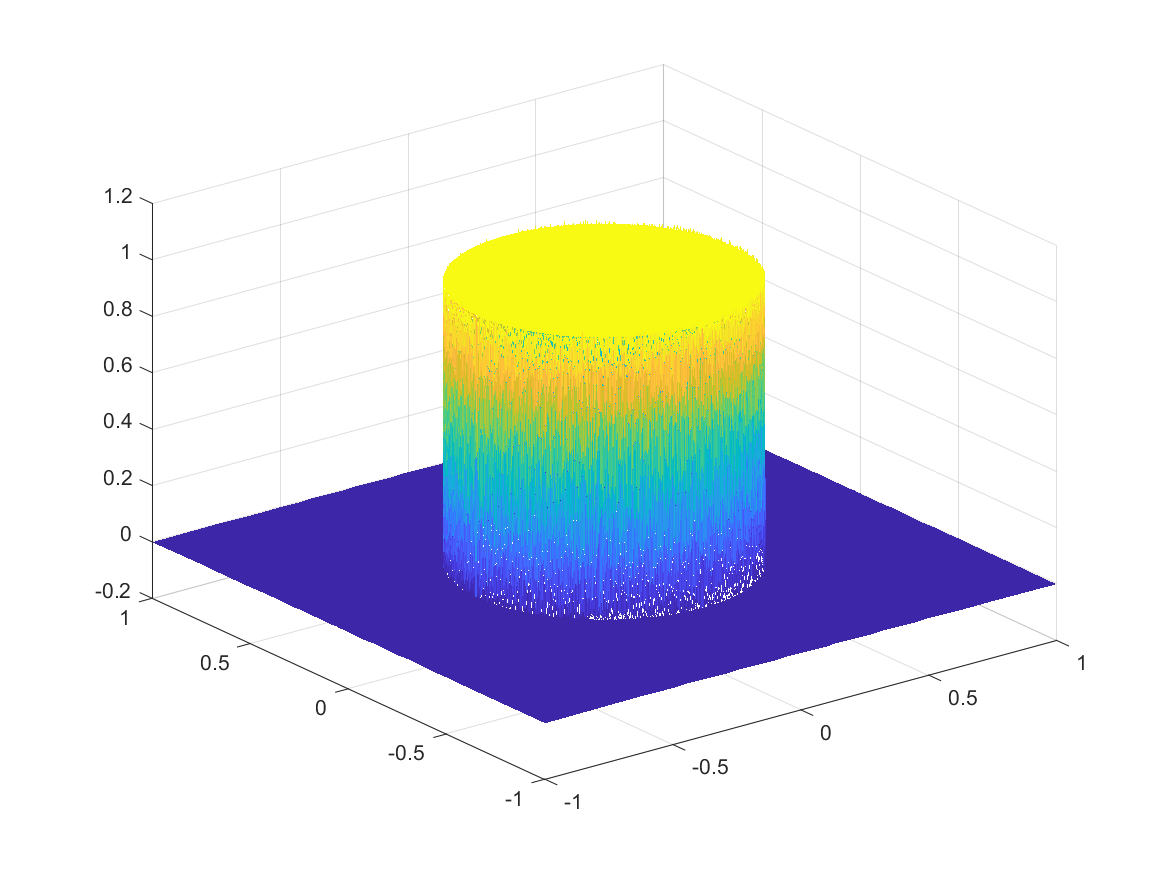
\includegraphics[trim = 40 30 30 30, clip, width=\linewidth]
      {pictures/chapExperiments/secGrayscale/circ/cont/adaptive/lvl28/solution.png}
    \label{fig:circContSol}
  \end{subfigure}
  \quad
  \begin{subfigure}[b]{.48\linewidth}
    \centering
    \caption{Lösung für $\fc$ entlang der Achsen}
    \includegraphics[trim = 50 30 50 20, clip, width=\linewidth]
      {pictures/chapExperiments/secGrayscale/circ/cont/adaptive/lvl28/solutionAxis.png}
    \label{fig:circContSolAxis}
  \end{subfigure}

  \begin{subfigure}[b]{.48\linewidth}
    \centering
    \caption{Lösung für $\fdc$}
    \includegraphics[trim = 40 30 30 30, clip, width=\linewidth]
      {pictures/chapExperiments/secGrayscale/circ/disc/adaptive/lvl26/solution.png}
    \label{fig:circDiscSol}
  \end{subfigure}
  \quad
  \begin{subfigure}[b]{.48\linewidth}
    \centering
    \caption{Lösung für $\fdc$ entlang der Achsen}
    \includegraphics[trim = 50 30 50 20, clip, width=\linewidth]
      {pictures/chapExperiments/secGrayscale/circ/disc/adaptive/lvl26/solutionAxis.png}
    \label{fig:circDiscSolAxis}
  \end{subfigure}
  \caption{Diskrete Lösungen sowie deren Darstellungen entlang der x-Achse
    (blau) und der y-Achse (rot) nach den Rechnungen mit den Eingangssignalen
    $\fc$ und $\fdc$}
  \label{fig:circleSol}
\end{figure}
Außerdem ähneln die in \Cref{fig:circleSol} dargestellten diskreten Lösungen der
Rechnungen mit den Eingangssignalen $\fc$ und $\fdc$ beide der exakten Lösung
für das Eingangssignal $f_\textup{C}$ aus \Cref{fig:circContExactSolAxis}.
Insgesamt scheinen sich die vergleichbaren Ergebnisse der Experimente mit den
Eingangssignalen $\fc$ und $\fdc$ tatsächlich kaum zu unterscheiden.
Entsprechend möchten wir nun die Experimente mit Eingangssignal $f_\textup{C}$
untersuchen und gehen davon aus, dass die folgenden Beobachtungen ähnlich auch 
für Experimente mit Eingangssignal $\fdc$ gültig sind.
\begin{figure}[p]
  \centering
  \includegraphics[width=.8\linewidth]
    {pictures/chapExperiments/secGrayscale/circ/convCont.pdf}
  \caption{Ergebnisse der Rechnungen mit adaptiver und uniformer 
    Netzverfeinerung für das Eingangssignal $\fc$}
  \label{fig:circContConvergence}
\end{figure}
In \Cref{fig:circContConvergence} ist zu sehen, dass bei diesem Experiment die
AFEM-Routine für die Fehlergraphen und den Anteil $\etaJ$ des
Verfeinerungsindikators mit adaptiver Netzverfeinerung bessere Konvergenzraten
erzielt als mit uniformer Netzverfeinerung.
Bei adaptiver Netzverfeinerung sind die entsprechenden Konvergenzraten etwa 1,
wobei die Rate für die Fehlergraphen sogar etwas größer zu sein scheint, und
bei uniformer Netzverfeinerung sind die Raten circa 1/2.
Dies wird bei diesem Beispiel daran liegen, dass eine starke Netzverfeinerung
bei der Unstetigkeit hier sinnvoller ist als eine Verfeinerung dort,
wo die Lösung konstant ist.
Der Verfeinerungsindikator $\etaT$ und sein Anteil $\etaV$, jeweils mit Rate 1,
sowie die von $\Egleb$ abhängigen Graphen, beide mit Rate 1/2, scheinen bei
uniformer und adaptiver Netzverfeinerung zwar die gleichen Raten zu haben, aber
bei adaptiver Netzverfeinerung deutlich geringere Werte zu erreichen.
Ansonsten ähnelt das Konvergenzverhalten, insbesondere bei uniformer 
Netzverfeinerung, dem bereits beim Experiment mit Eingangssignal $f_{10^4}$
in \Cref{fig:f01LargeAlphaConvergence} beobachteten.
Dies scheint daran zu liegen, dass dort ebenfalls $\alpha=10^4$ gewählt wurde.
Abschließend können wir betonen, dass Experimente existieren, bei denen
adaptive Netzverfeinerung ein besseres Konvergenzverhalten bewirkt als
uniforme.
\begin{figure}[p]
  \centering
  \begin{subfigure}{.32\linewidth}
    \centering
    \caption{$f_\textup{C}$}
    \includegraphics[width=\linewidth]
      {pictures/chapExperiments/secGrayscale/circ/misc.pdf}
    \label{fig:miscCircle}
  \end{subfigure}
  \begin{subfigure}{.32\linewidth}
    \centering
    \caption{$f_1$}
    \includegraphics[width=\linewidth]
      {pictures/chapExperiments/secExactSol/f01/misc.pdf}
    \label{fig:miscF01}
  \end{subfigure}
  \begin{subfigure}{.32\linewidth}
    \centering
    \caption{\texttt{cameraman}}
    \includegraphics[width=\linewidth]
      {pictures/chapExperiments/secGrayscale/cam/misc.pdf}
    \label{fig:miscCam}
  \end{subfigure}
  \caption{Anzahl der Iterationen und benötigte Zeit für die primalen-dualen
    Iterationen während des AFEM-Algorithmus bei den Rechnungen
    mit den Eingangssignalen $\fc$, $f_1$ und \texttt{cameraman}}
  \label{fig:miscInSi}
\end{figure}
Allerdings möchten wir an dieser Stelle auch festhalten, dass der adaptive
Algorithmus in den hier betrachteten Experimenten mehr Level durchläuft als der
Algorithmus mit uniformer Netzverfeinerung und für Iterationen auf
Triangulierungen mit vergleichbar vielen Freiheitsgaden in der Regel mehr
Iterationsschritte ausführt. 
Insgesamt benötigt ein Experiment bei adaptiver Netzverfeinerung also mehr Zeit
als bei uniformer Netzverfeinerung, wie in \Cref{fig:miscInSi} für drei
Eingangssignale und insbesondere das Eingangssignal $f_\textup{C}$ zu sehen
ist.


\section{Fazit und Ausblick}

Wir konnten in dieser Arbeit die Konvergenz der primalen-dualen Iteration nach
\cite{Bar15} für eine nichtkonforme, mit
Crouzeix-Raviart-Finite-Elemente-Funktionen diskretisierte Formulierung des
ROF-Modellproblems beweisen, den AFEM-Algorithmus mit dieser Iteration im
Solve-Schritt implementieren und in numerischen Experimenten
untersuchen. 
Dabei konnten wir die garantierte Rate für das in \cite{Bar15} betrachte
Problem übertreffen, auch wenn hierbei angemerkt werden muss, dass
wir in den entsprechenden Beispielen regulärere Eingangssignale und exakte
Lösungen betrachtet haben als lediglich Funktionen beschränkter Variation.
Weiterhin konnten wir im Vergleich zu uniformer Netzverfeinerung die
Verbesserung einiger Konvergenzraten bei adaptiver Netzverfeinerung für ein
Problem feststellen, bei dem die Unstetigkeitsmenge des Eingangssignals entlang
einer Teilmenge niedrigerer Dimension verlief, beziehungsweise ein
lokal betragsgroßer schwacher Gradient in der stetigen Approximation des
Eingangssignals auftrat, während dieses ansonsten nur konstante Werte annahm.
Allerdings ging die Verbesserung der Ergebnisse bei adaptiver Netzverfeinerung
mit einer erhöhten Rechenzeit einher.
Ist Rechenzeit kein limitierender Faktor, dann ist dementsprechend davon
auszugehen, dass bei solchen Experimenten adaptive Netzverfeinerung zu 
bevorzugen ist.
Die durch den benutzten Verfeinerungsindikator entstandenen adaptiven Netze
entsprachen unseren Erwartungen und für dessen Konvergenzverhalten konnten
wir Erklärungen finden.
Außerdem konnten wir die Gültigkeit der Interpretation des ROF-Modellproblems
aus \Cref{chap:introduction} in mehreren Experimenten erkennen.
Beim Test unserer Implementation entwickelten wir die Hypothese, dass die Größe
der rechten Seite der Ungleichung \eqref{eq:nrIterationsInequality} die
benötigte Iterationzahl bis zum Erreichen des Abbruchkriteriums
\eqref{eq:terminationCriterion} für die primale-duale Iteration beeinflusst.
Demnach führt eine größere Wahl von $\tau$ und $\alpha$, wobei allerdings die
Wahl von $\alpha$ das betrachtete Experiment verändert, zu weniger Iterationen.
Diese Hypothese wird von unseren Beobachtungen zur Größe der Parameter $\tau$
und $\alpha$ gestützt.
Für die Wahl der Parameter $\gamma$ und $\epsstop$ konnten wir ebenfalls
Empfehlungen formulieren.
Weiterhin konnten theoretische Aussagen der Arbeit, insbesondere Ungleichung
\eqref{eq:expectedInequalities} zur Abschätzung des exakten Fehlers durch von
den garantierten Energieschranken abhängigen Ausdrücken, experimentell
bestätigt werden.

Zum Abschluss dieser Arbeit möchten wir noch mögliche nächste Schritte
beschreiben.
Zunächst kann das Programm erweitert werden, indem die Annahme, dass
stets Nullranddaten vorliegen, aufgehoben wird. 
Dieses ist an einigen Stellen, zum Beisiel beim Erstellen der rechten Seite des 
Gleichungssystems während der primalen-dualen Iteration, noch unter ebendieser
Annahme optimiert.
Durch diese Erweiterung kann unter anderem bei Bildern als Eingangssignal auf
das Hinzufügen eines Randes, um Nullranddaten zu garantieren, verzichtet
werden.
Weiterhin kann damit untersucht werden, ob für die Geometrie \texttt{Lshape}
des AFEM-Softwarepakets ein Beispiel existiert, bei 
dem mit adaptiver Netzerfeinerung stark an der einspringenden Ecke verfeinert 
wird. 
In der aktuellen Implementation wird bei Eingangssignalen ohne Nullranddaten
an allen Kanten gleichermaßen verfeinert.
Als Nächstes kann die Implementierung der primalen-dualen Iteration für die
konforme Formulierung des ROF-Modellproblems aus \cite{Bar15} angepasst werden,
um deren Ergebnisse besser mit den Resultaten unserer Implementierung 
vergleichen zu können.
Kann für die Implementierung in \cite{Bar15} außerdem ein
Verfeinerungsindikator gefunden werden, so könnte diese ebenfalls im Rahmen des
AFEM-Algorithmus realisiert werden, um das Konvergenzverhalten zu vergleichen.
In der Theorie bleibt vor allem interessant, garantierte Konvergenzraten für
unsere Implementierung zu beweisen.
Zu diesem Zweck wäre die Konstruktion eines Beispiels mit bekannter
exakter Lösung und einem Eingangssignal, welches von beschränkter Variation und
nicht schwach differenzierbar ist, wichtig, um auch die Konvergenzraten
für ein weniger reguläres Beispiel sehen zu können.
Abschließend könnte auch die Wahl der Paramters $\tau$ weiter untersucht
werden, denn die Frage, ob es sinnvolle Möglichkeiten gibt, $\tau$ nicht
konstant zu wählen, bleibt offen.
Damit könnte eventuell das Konvergenzverhalten der Iteration verbessert und
somit die Anzahl der benötigten Iterationsschritte verringert werden.  Außerdem
könnte die Toleranz $\epsstop$ für das Abbruchkriterium zum Beispiel abhängig
von der Netzweite der Triangulierung gewählt werden, um sowohl die in einem
Experiment dieser Arbeit beobachtete Stagnation des exakten Fehlers zu
verhindern als auch die Iteration eines Levels nicht länger auszuführen als
notwendig.
